\documentclass[]{book}
\usepackage{lmodern}
\usepackage{amssymb,amsmath}
\usepackage{ifxetex,ifluatex}
\usepackage{fixltx2e} % provides \textsubscript
\ifnum 0\ifxetex 1\fi\ifluatex 1\fi=0 % if pdftex
  \usepackage[T1]{fontenc}
  \usepackage[utf8]{inputenc}
\else % if luatex or xelatex
  \ifxetex
    \usepackage{mathspec}
  \else
    \usepackage{fontspec}
  \fi
  \defaultfontfeatures{Ligatures=TeX,Scale=MatchLowercase}
\fi
% use upquote if available, for straight quotes in verbatim environments
\IfFileExists{upquote.sty}{\usepackage{upquote}}{}
% use microtype if available
\IfFileExists{microtype.sty}{%
\usepackage{microtype}
\UseMicrotypeSet[protrusion]{basicmath} % disable protrusion for tt fonts
}{}
\usepackage[margin=1in]{geometry}
\usepackage{hyperref}
\hypersetup{unicode=true,
            pdftitle={Análisis Estadístico de Datos Financieros con R},
            pdfauthor={Oswaldo Navarrete Carreño},
            pdfborder={0 0 0},
            breaklinks=true}
\urlstyle{same}  % don't use monospace font for urls
\usepackage{natbib}
\bibliographystyle{apalike}
\usepackage{color}
\usepackage{fancyvrb}
\newcommand{\VerbBar}{|}
\newcommand{\VERB}{\Verb[commandchars=\\\{\}]}
\DefineVerbatimEnvironment{Highlighting}{Verbatim}{commandchars=\\\{\}}
% Add ',fontsize=\small' for more characters per line
\usepackage{framed}
\definecolor{shadecolor}{RGB}{248,248,248}
\newenvironment{Shaded}{\begin{snugshade}}{\end{snugshade}}
\newcommand{\KeywordTok}[1]{\textcolor[rgb]{0.13,0.29,0.53}{\textbf{#1}}}
\newcommand{\DataTypeTok}[1]{\textcolor[rgb]{0.13,0.29,0.53}{#1}}
\newcommand{\DecValTok}[1]{\textcolor[rgb]{0.00,0.00,0.81}{#1}}
\newcommand{\BaseNTok}[1]{\textcolor[rgb]{0.00,0.00,0.81}{#1}}
\newcommand{\FloatTok}[1]{\textcolor[rgb]{0.00,0.00,0.81}{#1}}
\newcommand{\ConstantTok}[1]{\textcolor[rgb]{0.00,0.00,0.00}{#1}}
\newcommand{\CharTok}[1]{\textcolor[rgb]{0.31,0.60,0.02}{#1}}
\newcommand{\SpecialCharTok}[1]{\textcolor[rgb]{0.00,0.00,0.00}{#1}}
\newcommand{\StringTok}[1]{\textcolor[rgb]{0.31,0.60,0.02}{#1}}
\newcommand{\VerbatimStringTok}[1]{\textcolor[rgb]{0.31,0.60,0.02}{#1}}
\newcommand{\SpecialStringTok}[1]{\textcolor[rgb]{0.31,0.60,0.02}{#1}}
\newcommand{\ImportTok}[1]{#1}
\newcommand{\CommentTok}[1]{\textcolor[rgb]{0.56,0.35,0.01}{\textit{#1}}}
\newcommand{\DocumentationTok}[1]{\textcolor[rgb]{0.56,0.35,0.01}{\textbf{\textit{#1}}}}
\newcommand{\AnnotationTok}[1]{\textcolor[rgb]{0.56,0.35,0.01}{\textbf{\textit{#1}}}}
\newcommand{\CommentVarTok}[1]{\textcolor[rgb]{0.56,0.35,0.01}{\textbf{\textit{#1}}}}
\newcommand{\OtherTok}[1]{\textcolor[rgb]{0.56,0.35,0.01}{#1}}
\newcommand{\FunctionTok}[1]{\textcolor[rgb]{0.00,0.00,0.00}{#1}}
\newcommand{\VariableTok}[1]{\textcolor[rgb]{0.00,0.00,0.00}{#1}}
\newcommand{\ControlFlowTok}[1]{\textcolor[rgb]{0.13,0.29,0.53}{\textbf{#1}}}
\newcommand{\OperatorTok}[1]{\textcolor[rgb]{0.81,0.36,0.00}{\textbf{#1}}}
\newcommand{\BuiltInTok}[1]{#1}
\newcommand{\ExtensionTok}[1]{#1}
\newcommand{\PreprocessorTok}[1]{\textcolor[rgb]{0.56,0.35,0.01}{\textit{#1}}}
\newcommand{\AttributeTok}[1]{\textcolor[rgb]{0.77,0.63,0.00}{#1}}
\newcommand{\RegionMarkerTok}[1]{#1}
\newcommand{\InformationTok}[1]{\textcolor[rgb]{0.56,0.35,0.01}{\textbf{\textit{#1}}}}
\newcommand{\WarningTok}[1]{\textcolor[rgb]{0.56,0.35,0.01}{\textbf{\textit{#1}}}}
\newcommand{\AlertTok}[1]{\textcolor[rgb]{0.94,0.16,0.16}{#1}}
\newcommand{\ErrorTok}[1]{\textcolor[rgb]{0.64,0.00,0.00}{\textbf{#1}}}
\newcommand{\NormalTok}[1]{#1}
\usepackage{longtable,booktabs}
\usepackage{graphicx,grffile}
\makeatletter
\def\maxwidth{\ifdim\Gin@nat@width>\linewidth\linewidth\else\Gin@nat@width\fi}
\def\maxheight{\ifdim\Gin@nat@height>\textheight\textheight\else\Gin@nat@height\fi}
\makeatother
% Scale images if necessary, so that they will not overflow the page
% margins by default, and it is still possible to overwrite the defaults
% using explicit options in \includegraphics[width, height, ...]{}
\setkeys{Gin}{width=\maxwidth,height=\maxheight,keepaspectratio}
\IfFileExists{parskip.sty}{%
\usepackage{parskip}
}{% else
\setlength{\parindent}{0pt}
\setlength{\parskip}{6pt plus 2pt minus 1pt}
}
\setlength{\emergencystretch}{3em}  % prevent overfull lines
\providecommand{\tightlist}{%
  \setlength{\itemsep}{0pt}\setlength{\parskip}{0pt}}
\setcounter{secnumdepth}{5}
% Redefines (sub)paragraphs to behave more like sections
\ifx\paragraph\undefined\else
\let\oldparagraph\paragraph
\renewcommand{\paragraph}[1]{\oldparagraph{#1}\mbox{}}
\fi
\ifx\subparagraph\undefined\else
\let\oldsubparagraph\subparagraph
\renewcommand{\subparagraph}[1]{\oldsubparagraph{#1}\mbox{}}
\fi

%%% Use protect on footnotes to avoid problems with footnotes in titles
\let\rmarkdownfootnote\footnote%
\def\footnote{\protect\rmarkdownfootnote}

%%% Change title format to be more compact
\usepackage{titling}

% Create subtitle command for use in maketitle
\newcommand{\subtitle}[1]{
  \posttitle{
    \begin{center}\large#1\end{center}
    }
}

\setlength{\droptitle}{-2em}

  \title{Análisis Estadístico de Datos Financieros con R}
    \pretitle{\vspace{\droptitle}\centering\huge}
  \posttitle{\par}
    \author{Oswaldo Navarrete Carreño}
    \preauthor{\centering\large\emph}
  \postauthor{\par}
      \predate{\centering\large\emph}
  \postdate{\par}
    \date{A quién aún no ha visto la luz y ya ilumina mi vida.}

\ifxetex
  \usepackage{polyglossia}
  \setmainlanguage{spanish}
  \usepackage{longtable}
  % Tabla en lugar de cuadro
  \gappto\captionsspanish{\renewcommand{\tablename}{Tabla}  
          \renewcommand{\listtablename}{Índice de tablas}}
\else
  \usepackage[spanish,es-tabla]{babel}
  \usepackage{longtable}
\fi

\begin{document}
\maketitle

{
\setcounter{tocdepth}{1}
\tableofcontents
}
\chapter{¿A quién va dirigido este
libro?}\label{a-quien-va-dirigido-este-libro}

Este libro no es una introducción a la estadística. En la presente obra
se intenta hacer un repaso de algunos temas de estadistica que debe
conocer quien desee hacer investigación en Contabilidad, en Auditoría o
quizás en alguna ciencia social. Es probable que se omitan algunas cosas
pero la retroalimentación de los lectores de esta obra será importante
para su crecimiento.

En este texto se presentan, discuten y aplican los conceptos. La
presentación de los conceptos es realizada pensando en un diálogo entre
el autor y el lector, sin descuidar la formalidad de las expresiones
matemáticas. Para la discusión y aplicación de los conceptos, se va
mostrando al usuario como implementar el análisis estadístico en R.

Para aprovechar al máximo este libro se recomienda tener a mano una
computadora con R instalado, a fin de poder ir ejecutando los códigos
que se muestran. Los scripts y los conjuntos de datos que se presentan
pueden ser descargados de \url{https://github.com/oswnavarre/AEDFCR}

Aunque la obra tiene un enfoque práctico, el lector no debe olvidar que
aprender a usar R no implica saber estadística y que los programas
estadísticos no brindan soluciones si el usuario no conoce los conceptos
que deben ser aplicados.

\section{Instalando R Y Rstudio}\label{instalando-r-y-rstudio}

R es un lenguaje y entorno para computación estadística y gráficos. En
los últimos años el uso del programa estadístico R ha ido en aumento.
Puede ser descargado de \url{https://cran.r-project.org/}. Una de las
características interesantes del programa es que su capacidad puede ser
incrementada con la ayuda de paquetes, en la actualidad la página
oficial del programa tiene cerca de 14000 paquetes.

RStudio es una interfaz que ayuda a explotar todas las capacidades de R.
Rstudio se descarga de la página \url{https://www.rstudio.com/}.

\chapter{Introducción}\label{intro}

En nuestra vida diaria es común escuchar el término
\textbf{estadística}, las tasas de desempleo, el índice de pobreza, el
saldo promedio de nuestra cuenta de ahorros, el número de goles
realizados en la LigaPro durante el fin de semana, etc. Aunque no es una
forma incorrecta de ver las estadísticas, en este texto se pensará a la
estadística como un conjunto de métodos que se utilizan para
\textbf{recoger, clasificar, resumir, organizar, presentar, analizar e
interpretar información numérica}

En las empresas la estadística es usada para tomar decisiones como los
productos y las cantidades que deben ser producidas, la frecuencia con
la que una maquinaria debe recibir mantenimiento, el tamaño del
inventario, la forma de distribuir los productos, y casi todos los
aspectos relativos a sus operaciones. En el estudio de las finanzas, la
contabilidad, la economía y otras ciencias sociales la motivación para
usar estadística radica en entender como funcionan los sistemas
económicos, financieros o contables.

\section{Estadística descriptiva e inferencial}\label{estypes}

El uso de la estadística puede ser de dos formas. La primera, cuando se
describen y se presentan los datos. Y la segunda es cuando los datos son
utilizados para hacer inferencias sobre características del ambiente o
entorno de donde se seleccionaron los datos o sobre el mecanismo
subyacente que generó los datos. La primera forma recibe el nombre de
\textbf{estadística descriptiva} y la segunda se conoce como
\textbf{estadística inferencial}

En la estadística descriptiva se utilizan métodos numéricos y gráficos
para encontrar patrones y características de los datos a fin de resumir
la información y presentarla de una forma significativa. Mientras que en
la estadística inferencial se utilizan los daots para tomar decisiones,
hacer estimaciones, pronósticos o predicciones y generalizaciones sobre
el entorno del que fueron obtenidos los datos o el proceso que los
generó.

Sea en estadística descriptiva o en estadística inferencial, el primer
paso siempre va a ser obtener información de alguna característica,
medida o valor que nos interese de un grupo de elementos. Esa
característica, medida o valor de interés para el investigador recibe el
nombre de \textbf{variable}.

\section{Tipos de Variables}\label{tipos-de-variables}

Muchos autores presentan algunas clasificaciones para las variables, sin
embargo vamos a trabajar con una clasificación que se ajusta a las
necesidades de la investigación en las áreas de nuestro interés. Según
esta clasificación hay dos grandes grupos de variables: cuantitativas y
cualitativas. Las primeras son las que toman valores \textbf{numéricos}.
Mientras que las cualitativas toman valores que describen una
\textbf{cualidad} o \textbf{característica}.

Las variables cuantitativas se clasifican a la vez en \textbf{continuas}
que se presentan cuando las observaciones pueden tomar cualquier valor
dentro de un subconjunto de los números reales, ejemplos de variables
cuantitativas continuas son: edad, altura, temperatura y peso. Las
\textbf{discretas} son aquellas cuya característica principal es que las
observaciones pueden tomar un valor basado en un recuento de un conjunto
de valores enteros distintos. Ejemplos de variables cuantitativas
discretas son: número de hijos, número de comprobantes de venta emitidos
en un mes, número de clientes haciendo fila durante una hora en un
banco.

\subsection{Niveles de medición}\label{niveles-de-medicion}

Hay cuatro niveles de medición \textbf{ordinal}, \textbf{nominal},
\textbf{intervalo} y de \textbf{radio}. En el nivel ordinal las
observaciones toman valores que se ordenan o clasifican de forma lógica,
por ejemplo las tallas de ropa (pequeña, media, grande, extra grande),
la frecuencia con la que se hace una actividad (nunca, casi nunca, a
veces, casi siempre, siempre). Por otro lado, en el nivel nominal las
observaciones toman valores que no se pueden organizar de forna lógica,
por ejemplo el sexo, el color de ojos, la marca de ropa favorita.

En el nivel de intervalo existe diferencia significativa entre valores
pero el cero no representa la ausencia de la característica un ejemplo
es la temperatura medida en grados Farenheit. Finalmente en el nivel de
razón el 0 es significativo y la razón entre dos números es
significativa, un ejemplo es la temperatura medida en grados Kelvin.

\section{Otros conceptos importantes}\label{otros-conceptos-importantes}

Existen algunos conceptos que son importantes y que se deben tener
presentes en el análisis estadístico de datos.

\begin{itemize}
\tightlist
\item
  \textbf{Población}: una población es el conjunto de todos los sujetos
  u objetos de interés en una investigación o análisis. Por ejemplo si
  se desea analizar la intención de voto en una ciudad para las próximas
  elecciones seccionales, la población serían todas las personas en edad
  de votar empadronadas en la ciudad.
\item
  \textbf{Muestra}: es la parte de la población que es analizada.
  Sigamos con el ejemplo de la intención de voto, aunque el investigador
  quisiera no puede acceder a toda la población ya sea por cuestiones de
  tiempo o dinero y por esta razón debe tomar una parte de la población.
  La muestra debe representar lo mejor posible a la población. La parte
  de la estadística que comprende los métodos estadísticos para obtener
  muestras representativas de una población se llama \emph{muestreo}
\item
  \textbf{Parámetro}: un parámetro es una cantidad numérica que
  caracteriza a una población.
\item
  \textbf{Estadístico}: un estadístico es una cantidad numérica que
  caracteriza a una muestra.
\end{itemize}

\section{Primeros pasos en R}\label{primerR}

Una vez instalado R y RStudio, abrimos Rstudio para comenzar a trabajar.
La ventana de RStudio se ve como se muestra en la figura
\ref{fig:rstudio1}.

\begin{figure}[h]

{\centering 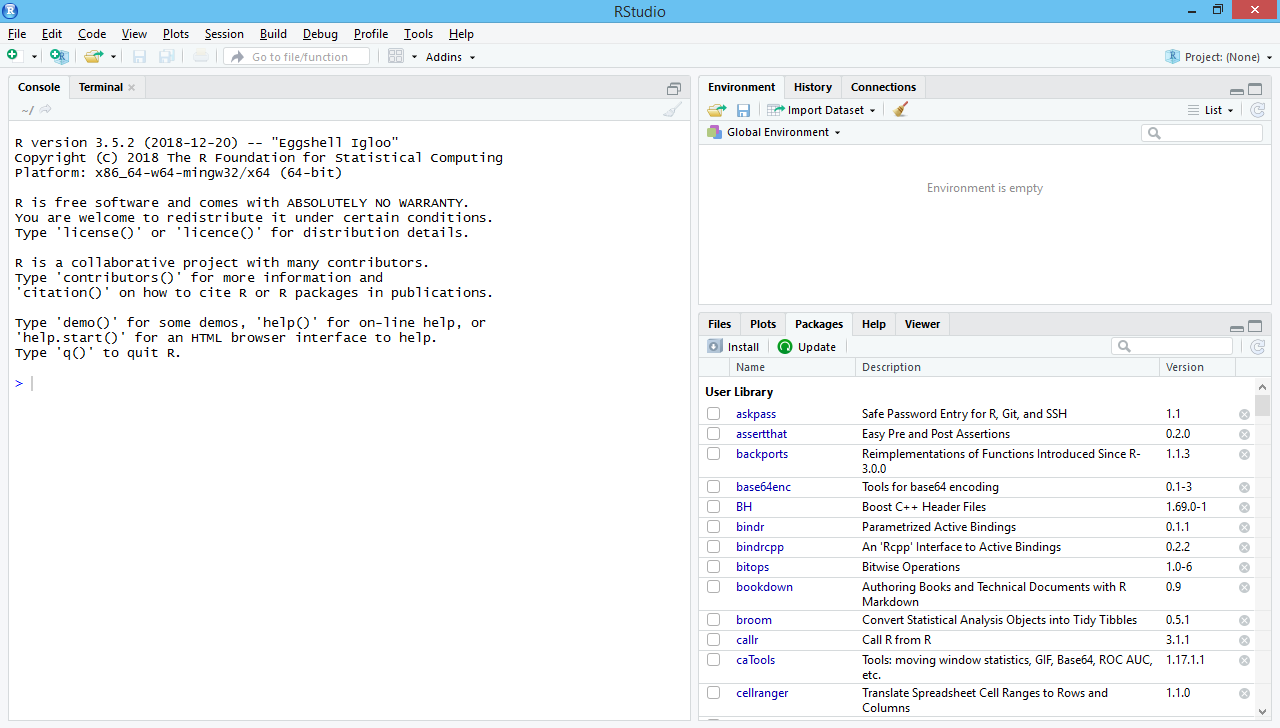
\includegraphics[width=0.5\linewidth]{rstudio1} 

}

\caption{Ventana de RStudio}\label{fig:rstudio1}
\end{figure}

Lo primero que debemos hacer es abrir un nuevo script, un script de R es
simplemente un archivo de texto que contiene (casi) todos los comandos
que se escribirían en la línea de comandos de R, para esto en la barra
de menú seguimos la secuencia \textbf{File, New File, R Script} o desde
el teclado con la combinación \emph{Ctrl + Shift + N}, en este archivo
iremos escribiendo todos los comandos que vamos a trabajar. En la figura
\ref{fig:rstudio2} se aprecia un script abierto.

\begin{figure}[h]

{\centering 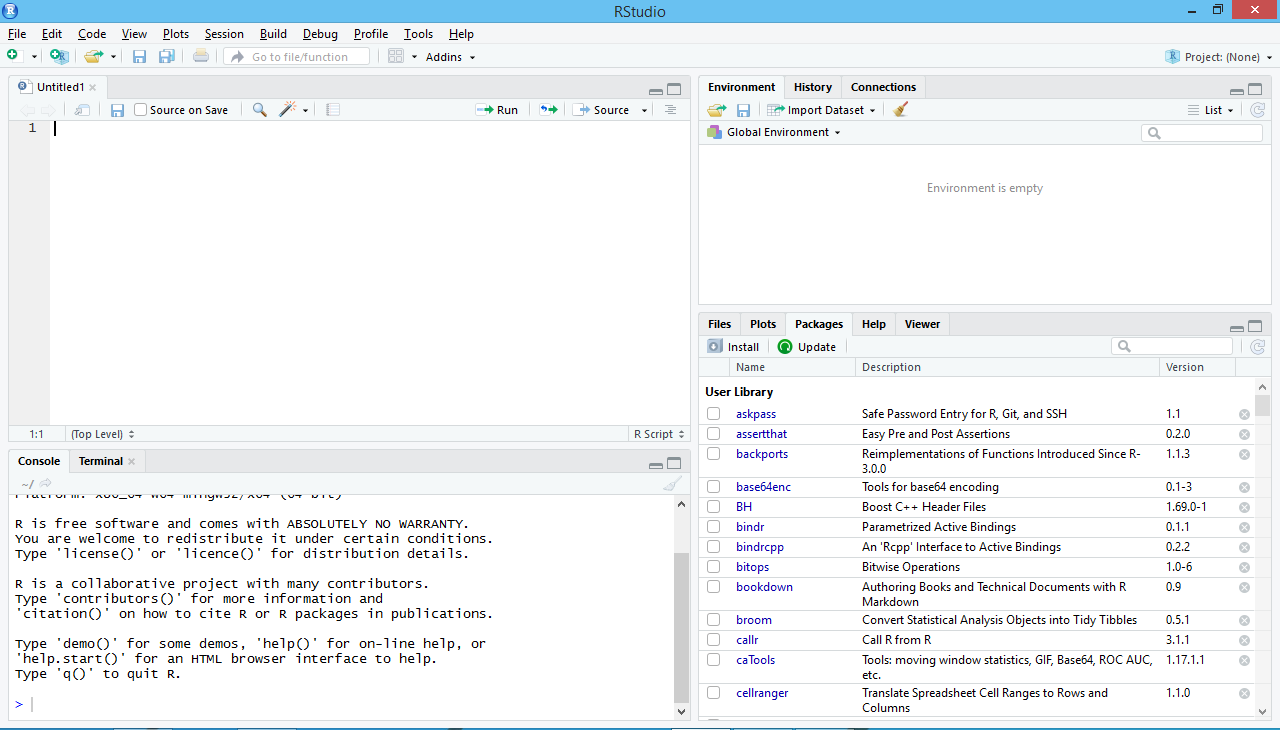
\includegraphics[width=0.5\linewidth]{rstudio2} 

}

\caption{Ventana de RStudio con Script}\label{fig:rstudio2}
\end{figure}

Para empezar a aprender en el script vamos a escribir \texttt{3+2} y
ejecutamos esto con la combinación de teclas \textbf{Ctrl + Enter} el
resultado obviamente es 5. Ahora ingresaremos un conjunto de valores y
los almacenaremos en una variable, para almacenar algo en una variable
se puede usar \texttt{\textless{}-} o \texttt{=}. En la variable
\texttt{x} almacenaremos un conjunto de 8 observaciones escribiendo el
código:

\begin{Shaded}
\begin{Highlighting}[]
\NormalTok{x <-}\StringTok{ }\KeywordTok{c}\NormalTok{(}\DecValTok{3}\NormalTok{,}\DecValTok{7}\NormalTok{,}\DecValTok{9}\NormalTok{,}\DecValTok{5}\NormalTok{,}\DecValTok{6}\NormalTok{,}\DecValTok{2}\NormalTok{,}\DecValTok{1}\NormalTok{,}\DecValTok{10}\NormalTok{) }
\end{Highlighting}
\end{Shaded}

Recuerde que este código se ejecuta con la combinación de teclas
\textbf{Ctrl + Enter}. Para poder realizar análisis estadístico, es
necesario cargar nuestros datos en el programa. R acepta algunos
formatos de archivos, como por ejemplo archivos de Excel, archivos de
valores separados por coma, archivos de texto e inclusive archivos de
otros programas como SPSS. Lo más usual es trabajar con archvo de
valores separados por coma es decir con extensión \texttt{.csv}, estos
archivos \texttt{csv} se generan cuando el investigador recolecta la
información, la almacena en un archivo de Excel o alguna otra hoja de
cálculo y la guarda como un archivo de valores separados por coma.

Para trabajar de forma eficiente con R, se recomienda comenzar por fijar
un directorio de trabajo donde deben estar guardados nuestros archivos
en el formato que sea de nuestra preferencia. Una forma de hacerlo es
desde la barra de menú \textbf{Session, Set Working Directory, Choose
Directory} o desde el teclado con la combinación \textbf{Ctrl+Shift+H},
o con la función \texttt{setwd("rutadelarchivo")}.

En este primer ejercicio trabajaremos con el archivo
\emph{cap2\_big4\_size.csv}. Los datos serán guardados en una variable
llamada \texttt{datos1}, usaremos la función \texttt{read.csv()} para
leer los datos. La función \texttt{read.csv()} recibe las instrucciones
\texttt{read.csv("archivo",\ header=T,\ sep=";",dec=",")}. La opción
\texttt{"archivo"} indica el nombre del archivo, \texttt{header=T} o
\texttt{header=F} permite indicar si las columnas tienen un encabezado
que las identifique, \texttt{sep=";"} sirve para indicar cual es el
separador presente en nuestro archivo en algunas ocasiones ocurre que un
archivo de valores separado por coma en realidad tiene sus valores
separados por un punto y cona esto generalmente ocurre cuando el sistema
utiliza, como en este caso, la coma como separador decimal y finalmente
la opción \texttt{dec=","} sirve para indicar que el separador decimal
es la coma.

Una característica de R es que permite acceder a la ayuda sobre las
funciones, esto se hace escribiendo \texttt{?funcion} por ejemplo si
queremos la ayuda de la función \texttt{read.csv} simplemente escribimos
\texttt{?read.csv} en el panel ubicado en la parte inferior derecha se
desplegará la ayuda de la función. Con la particularidad de que la ayuda
se despliega en inglés lo que no debería ser problema para un buen
investigador.

El archivo que vamos a analizar contiene los activos, la utilidad, las
ventas y el patrimonio de una muestra de empresas tomada de los
registros de la Superintendencia de Compañías. Además en el conjunto de
datos se indica si la empresa ha sido auditada por una de las 4 firmas
auditoras consideradas las más grandes o también llamadas
\emph{\emph{Big Four}}. En la \ref{tab:tabla1} se muestran las 10
primeras observaciones de nuestro conjunto de datos.

\label{tab:tabla1}Primeras 10 observaciones

EXPMUESTRA

BIG4

ACTIVOS

UTILIDAD

VTAS

PAT

85

1

73315618

7522758.7

191474544

39382529

100121

0

21052702

-122898.5

132585022

1577764

45178

0

10468672

536876.9

13974269

4312094

51193

0

4130483

455759.4

8670153

1858990

47598

0

23507401

266370.5

18555609

7137609

31720

0

7220312

437718.3

16097135

4002154

46189

0

14526822

1206400.9

12281188

5015806

9731

0

8539445

367848.1

10844918

2232339

4619

0

2605059

-22438.4

6244589

1366610

102434

0

23975816

790265.6

40612649

8754369

Sin más preámbulos, empecemos a trabajar. Recapitulando, primero
configuraremos el directorio de trabajo, luego cargaremos el archivo
indicado. Finalmente usamos la función \texttt{str()}, la que nos
permite obtener la descripción de la estructura de los datos.

\begin{Shaded}
\begin{Highlighting}[]
\KeywordTok{setwd}\NormalTok{(}\StringTok{"C:/Users/onava_000/OneDrive/libro_mc/estadistica"}\NormalTok{)}
\NormalTok{big4size <-}\StringTok{ }\KeywordTok{read.csv}\NormalTok{(}\StringTok{"cap2_big4_size.csv"}\NormalTok{,}\DataTypeTok{header=}\OtherTok{TRUE}\NormalTok{,}\DataTypeTok{sep=}\StringTok{";"}\NormalTok{,}\DataTypeTok{dec=}\StringTok{","}\NormalTok{)}
\KeywordTok{str}\NormalTok{(big4size)}
\end{Highlighting}
\end{Shaded}

\begin{verbatim}
## 'data.frame':    2256 obs. of  6 variables:
##  $ EXPMUESTRA: int  85 100121 45178 51193 47598 31720 46189 9731 4619 102434 ...
##  $ BIG4      : int  1 0 0 0 0 0 0 0 0 0 ...
##  $ ACTIVOS   : num  73315618 21052702 10468672 4130483 23507401 ...
##  $ UTILIDAD  : num  7522759 -122898 536877 455759 266371 ...
##  $ VTAS      : num  1.91e+08 1.33e+08 1.40e+07 8.67e+06 1.86e+07 ...
##  $ PAT       : num  39382529 1577764 4312094 1858990 7137609 ...
\end{verbatim}

En la primera línea de los resultados se observa la salida
\texttt{\textquotesingle{}data.frame\textquotesingle{}:\ \ \ \ 2256\ obs.\ of\ \ 6\ variables:}
esto nos indica que nuestro \emph{marco de datos (data frame)} tiene
2256 observaciones y 6 variables. Con respecto a las variables tenemos 6
variables que a continuación se describen y se explican los resultados
obtenidos con la función.

\begin{itemize}
\tightlist
\item
  \texttt{EXPMUESTRA}: esta variable es de tipo entera (INT) y almacena
  el expediente de la empresa. Aunque la variable tiene valores
  numéricos, no es una variable cuantitativa sino cualitativa
  ``Expediente de la Empresa''
\item
  \texttt{BIG4}: esta variable es de tipo entera, y ha sido codificada
  con 1 si la empresa fue auditada por una Big Four y 0 si no. Podemos
  cambiar esta codificación por ``Sí'' y ``No'' en lugar de ``1'' y
  ``0'', más adelante aprendemos como hacerlo. Al igual que la variable
  anterior aunque tiene valores numéricos, no es una variable
  cuantitativa sino cualitativa, dejamos al lector la reflexión en este
  particular.
\item
  \texttt{ACTIVOS}: contiene el valor de los activos totales de la
  empresa. Es de tipo \texttt{num} porque permite el uso de decimales.
  Corresponde a una variable cuantitativa continua.
\item
  \texttt{UTILIDAD}: contiene el valor de la utildad de la empresa.
\item
  \texttt{VTAS}: contiene el valor de las ventas de la empresa.
\item
  \texttt{PAT}: contiene el valor del patrimonio de la empresa.
\end{itemize}

Los paquetes de R son colecciones de funciones y conjuntos de datos
desarrollados por la comunidad de usuarios, los paquetes aumentan el
poder de R mejorando las funcionalidades existentes en la base de R, o
añadiendo nuevas funcionalidades. En este texto trabajaremos con algunos
de los paquetes desarrollados por el equipo de RStudio, una descripción
detallada de estos paquetes puede ser encontrada en
\url{https://www.rstudio.com/products/rpackages/}. . Comenzaremos por
instalar el paquete \texttt{dplyr}, este paquete tiene funciones que
permiten realizar facilmente manipulaciones de datos. Para instalar un
paquete se utiliza la función \texttt{install.packages("paquete")}. Una
vez instalado el paquete, se carga el paquete utilizando la función
\texttt{library(paquete)}.

\begin{Shaded}
\begin{Highlighting}[]
\KeywordTok{install.packages}\NormalTok{(}\StringTok{"dplyr"}\NormalTok{)}
\end{Highlighting}
\end{Shaded}

La primera manipulación que vamos a realizar es la creación de nuevas
variables con el paquete \texttt{dplyr}. En nuestros datos cargados en
el conjunto de datos \texttt{datos1} vamos a crear tres variables nuevas
\textbf{ROA}, \textbf{ROS} y \textbf{ROE}. Recordemos que el
\textbf{Retorno sobre activos} ( \textbf{ROA}, Return on Assets) se lo
calcula como la razón entre la utilidad y los activos como se ve en la
ecuación \eqref{eq:roa}. En las ecuaciones \eqref{eq:ros} y \eqref{eq:roe} se
dan las expresiones para calcular el \textbf{Retorno sobre ventas} (
\textbf{ROS} Return on Sales) y el \textbf{Retorno sobre el Patrimonio}
( \textbf{ROE} Return on Equity)

\begin{equation} 
  ROA = \dfrac{Utilidad}{Activos}
  \label{eq:roa}
\end{equation}

\begin{equation} 
  ROS = \dfrac{Utilidad}{Ventas}
  \label{eq:ros}
\end{equation}

\begin{equation} 
  ROE = \dfrac{Utilidad}{Patrimonio}
  \label{eq:roe}
\end{equation}

Una característica importante de \texttt{dplyr} es el uso del operador
\texttt{\%\textgreater{}\%}. Cada transformación u operación en los
datos se separa por el operador \texttt{\%\textgreater{}\%}. La primera
función de \texttt{dplyr} que usaremos es \texttt{mutate()}, básicamente
esta función permite crear nuevas variables.

\begin{Shaded}
\begin{Highlighting}[]
\KeywordTok{library}\NormalTok{(dplyr)}
\NormalTok{big4size <-}\StringTok{ }\NormalTok{big4size }\OperatorTok
\StringTok{  }\KeywordTok{mutate}\NormalTok{(}
    \DataTypeTok{ROA =}\NormalTok{ UTILIDAD}\OperatorTok{/}\NormalTok{ACTIVOS,}
    \DataTypeTok{ROS =}\NormalTok{ UTILIDAD}\OperatorTok{/}\NormalTok{VTAS,}
    \DataTypeTok{ROE =}\NormalTok{ UTILIDAD}\OperatorTok{/}\NormalTok{PAT}
\NormalTok{  )}
\KeywordTok{str}\NormalTok{(big4size)}
\end{Highlighting}
\end{Shaded}

\begin{verbatim}
## 'data.frame':    2256 obs. of  9 variables:
##  $ EXPMUESTRA: int  85 100121 45178 51193 47598 31720 46189 9731 4619 102434 ...
##  $ BIG4      : int  1 0 0 0 0 0 0 0 0 0 ...
##  $ ACTIVOS   : num  73315618 21052702 10468672 4130483 23507401 ...
##  $ UTILIDAD  : num  7522759 -122898 536877 455759 266371 ...
##  $ VTAS      : num  1.91e+08 1.33e+08 1.40e+07 8.67e+06 1.86e+07 ...
##  $ PAT       : num  39382529 1577764 4312094 1858990 7137609 ...
##  $ ROA       : num  0.10261 -0.00584 0.05128 0.11034 0.01133 ...
##  $ ROS       : num  0.039289 -0.000927 0.038419 0.052566 0.014355 ...
##  $ ROE       : num  0.191 -0.0779 0.1245 0.2452 0.0373 ...
\end{verbatim}

En las últimas líneas de la salida de R, se observa que ahora en el
conjunto de datos existen ahora tres nuevas variables. En la próxima
sección seguiremos trabajando con el mismo conjunto de datos.

\section{Medidas de Tendencia
Central}\label{medidas-de-tendencia-central}

Una medida de tendencia central, es una medida de resumen que intenta
describir un conjunto completo de datos con un único valor que
representa la mitad o centro de la distribución.

Las tres medidas de tendencia central principales son la media la
mediana y la moda.

\subsection{Media}\label{media}

La media se la calcula como la suma de todos los valores de una variable
dividido para el número de valores. En la ecuación \eqref{eq:mean} se
muestra la fórmula para calcular la media.

\begin{equation} 
  \bar{x} = \dfrac{\sum_{i=1}^{n}x_i}{n}
  \label{eq:mean}
\end{equation}

La media tiene algunas propiedades que a continuación se detallan:

\begin{itemize}
\tightlist
\item
  Si a cada valor \(x_i\) de una distribución con media \(\bar{x}\) se
  le suma un valor constante \(k \in \mathbb{R}\), la nueva media es
  \(\bar{x}+k\)
\item
  Si a cada valor \(x_i\) de una distribución con media \(\bar{x}\) se
  lo multiplica por un valor constante \(k \in \mathbb{R}\), la nueva
  media es \(k\bar{x}\)
\item
  Si a cada valor \(x_i\) de una distribución con media \(\bar{x}\) se
  lo divide por un valor constante \(k \neq 0 \in \mathbb{R}\), la nueva
  media es \(\dfrac{\bar{x}}{k}\)
\end{itemize}

Las ventajas de usar la media son:

\begin{itemize}
\tightlist
\item
  Es fácil de entender y calcular
\item
  No se ve afectada mayormente por fluctuaciones productos del muestreo
\item
  Toma en cuenta todos los valores de la variable
\end{itemize}

Las desventajas de usar la media son:

\begin{itemize}
\tightlist
\item
  Es muy sensible a la presencia de pocos valores muy pequeños o muy
  grandes, dicho de otra forma la media es sensible a valores
  aberrantes.
\item
  No se puede calcular por inspección.
\end{itemize}

\subsection{Mediana}\label{mediana}

La mediana es el valor central en una distribución cuando se ordenan los
valores de forma ascendente o descendente. El valor de la mediana
depende entonces del número de valores presentes en la variable.
Definamos como \(\left\{ X \right \}\) al conjunto de datos ordenado, y
sea \(\left \{ X \right \}_i\) el valor i-ésimo del conjunto
\(\left \{ X \right \}\) entonces la mediana \(Me\) se define como

\begin{equation}
Me = \begin{cases} 
      \left \{ X \right\}_{\frac{n+1}{2}} & ; n \quad \textrm{impar}  \\
      \dfrac{\left \{ X  \right \}_{\frac{n}{2}} + \left \{ X  \right \}_{\frac{n}{2}+1} }{2} & ; n \quad \textrm{par}
   \end{cases}
   \label{eq:median}
\end{equation}

Lo escrito en la ecuación \eqref{eq:median} se puede expresar de la
siguiente forma: si el número de datos es impar, la mediana es igual al
valor central de la distribución y si el número de datos es par, la
mediana es igual al promedio de los valores centrales de la
distribución.

Las ventajas de usar la mediana son:

\begin{itemize}
\tightlist
\item
  Es fácil de calcular y comprender
\item
  No se ve afectada por valores extremos
\item
  Se puede determinar para escalas ordinales, nominales, de razón e
  intervalo
\end{itemize}

Las desventajas de usar la mediana son:

\begin{itemize}
\tightlist
\item
  No toma en cuenta el valor exacto de cada dato y por tanto no usa toda
  la información disponible.
\item
  Si se agrupan los valores de dos grupos, la mediana de cada grupo no
  puede ser expresada en términos del grupo agrupado.
\end{itemize}

\subsection{Moda}\label{moda}

La moda es definida como el valor que ocurre con mayor frecuencia en los
datos. Algunos conjuntos de datos no tienen moda porque cada valor
ocurre solo una vez. Hay conjuntos de datos que tienen más de una moda,
si tienen 2 modas reciben el nombre de bimodal y se acostumbra que si
tiene más de 3 modas se la llama multimodal.

Las ventajas de usar la moda son:

\begin{itemize}
\tightlist
\item
  Puede ser usada para datos con escala nominal
\item
  Es sencilla de calcular
\end{itemize}

La desventaja de la moda es:

\begin{itemize}
\tightlist
\item
  No es usada en análisis estadístico debido a que no está definida
  algebraicamente y la fluctuación en la frecuencia de las observaciones
  es mayor cuando el tamaño de la muestra es pequeña.
\end{itemize}

\subsection{¿trabajamos con la media o la
mediana?}\label{trabajamos-con-la-media-o-la-mediana}

La media es considerada generalmente la mejor medida de tendencia
central y la más usada. Sin embargo, hay situaciones donde las otras
medidas de tendencia central son preferidas.

La mediana es preferida a la media cuando:

\begin{itemize}
\tightlist
\item
  Hay valores extremos en la distribución
\item
  Hay valores indeterminados
\item
  Los datos son medidos en una escala ordinal
\end{itemize}

La moda es la medida preferida cuando los datos son medidos en una
escala nominal.

\subsection{Cálculo de las medidas de tendencia central en
R}\label{calculo-de-las-medidas-de-tendencia-central-en-r}

Para calcular la media y la mediana se utilizan las funciones
\texttt{mean()} y \texttt{median()} respectivamente, estas dos funciones
vienen cargadas con los paquetes base de R. Para calcular la moda
usaremos la función \texttt{Mode()} del paquete \texttt{DescTools},
recuerde que para instalar un paquete se utiliza la función
\texttt{install.packages()}.

En el siguiente ejemplo se obtiene la media de los activos de las
empresas. como solamente necesitamos una variable del conjunto de datos
usamos el operador \texttt{\$}, el funcionamiento de este operador es
\texttt{data.frame\$variable} es decir indicamos el conjunto de datos
del que llamamos la variable y después del operador \texttt{\$}
indicamos la variable que vamos a trabajar.

\begin{Shaded}
\begin{Highlighting}[]
\KeywordTok{mean}\NormalTok{(big4size}\OperatorTok{$}\NormalTok{ACTIVOS)}
\end{Highlighting}
\end{Shaded}

\begin{verbatim}
## [1] 44064165
\end{verbatim}

\begin{Shaded}
\begin{Highlighting}[]
\KeywordTok{median}\NormalTok{(big4size}\OperatorTok{$}\NormalTok{ACTIVOS)}
\end{Highlighting}
\end{Shaded}

\begin{verbatim}
## [1] 10326361
\end{verbatim}

\begin{Shaded}
\begin{Highlighting}[]
\KeywordTok{library}\NormalTok{(DescTools)}
\KeywordTok{Mode}\NormalTok{(big4size}\OperatorTok{$}\NormalTok{ACTIVOS)}
\end{Highlighting}
\end{Shaded}

\begin{verbatim}
## [1]  55996406 628446149
\end{verbatim}

En el resultado de la moda se obtienen 2 valores. Es decir que existen
dos valores que se repiten más veces o tienen mayor frecuencia. Cuando
se realiza investigación es común desear hacer una tabla con las
estadísticas descriptivas de los datos. El paquete \texttt{dplyr}
permite realizar tablas que resuman las variables de forma sencilla con
la función \texttt{summarise()}.

\begin{Shaded}
\begin{Highlighting}[]
\NormalTok{big4size }\OperatorTok
\StringTok{  }\KeywordTok{summarise}\NormalTok{(}\DataTypeTok{PROM.ACTIVOS =} \KeywordTok{mean}\NormalTok{(ACTIVOS),}
            \DataTypeTok{PROM.UTILIDAD =} \KeywordTok{mean}\NormalTok{(UTILIDAD),}
            \DataTypeTok{PROM.VTAS =} \KeywordTok{mean}\NormalTok{(VTAS),}
            \DataTypeTok{MEDIAN.ACTIVOS =} \KeywordTok{median}\NormalTok{(ACTIVOS),}
            \DataTypeTok{MEDIAN.UTILIDAD =} \KeywordTok{median}\NormalTok{(UTILIDAD),}
            \DataTypeTok{MEDIAN.VTAS =} \KeywordTok{median}\NormalTok{(VTAS)}
\NormalTok{            )}
\end{Highlighting}
\end{Shaded}

\begin{verbatim}
##   PROM.ACTIVOS PROM.UTILIDAD PROM.VTAS MEDIAN.ACTIVOS MEDIAN.UTILIDAD
## 1     44064165       4250664  50555030       10326361        350642.1
##   MEDIAN.VTAS
## 1     9190661
\end{verbatim}

\section{Medidas de posición
(Cuantiles)}\label{medidas-de-posicion-cuantiles}

Las medidas de posición no central permiten conocer otros puntos
característicos de la distribución que no son los valores centrales.
Entre las medidas de posición no central más importantes están los
cuantiles. El término cuantil fue usado por primera vez por Kendall en
1940.

El cuantil de orden p de una distribución con \(0<p<1\) es el valor
\(x_{i}\) de la variable \(X\) que marca un corte de modo que una
proporción \(p\) o un porcentaje \(100p\)\% de valores de la población
es menor o igual que \(x_{i}\) Por ejemplo el cuantil de orden \(0.35\)
dejaría un 35\% de valores por debajo de él.

\subsection{Tipos de Cuantiles}\label{tipos-de-cuantiles}

\begin{itemize}
\item
  \emph{Cuartiles}: son 3 valores (\(Q_{1}, Q_{2}, Q_{3}\)) que dividen
  a la distribución en 4 partes iguales.
\item
  \emph{Quintiles}: son 4 valores (\(K_{1}, K_{2}, K_{3}, K_{4}\)) que
  dividen a la distribución en 5 partes iguales.
\item
  \emph{Deciles}: son 9 valores
  (\(D_1, D_2, D_3, D_4, D_5, D_6, D_7, D_8, D_9\)) que dividen a la
  distribución en 10 partes iguales.
\item
  \emph{Percentiles}, son 99 valores (\(P_1, P_2, \ldots P_{99}\)) que
  dividen a la distribución en 100 partes iguales.
\end{itemize}

\subsection{Cálculo de cuantiles}\label{calculo-de-cuantiles}

Es fácil darse cuenta que existen equivalencias importantes entre los
cuantiles, algunos ejemplos de estas equivalencias:

\begin{itemize}
\tightlist
\item
  \(D_5=Q_2=P_{50}\)
\item
  \(D_4=K_2=P_{40}\)
\item
  \(D_3=P_{30}\)
\end{itemize}

Se deduce entonces que no es necesario tener una expresión para cada
tipo de cuantiles, basta con conocer una expresión para calcular
percentiles. Para esto debemos conocer dos cosas:

\begin{enumerate}
\def\labelenumi{\arabic{enumi}.}
\tightlist
\item
  La posición del percentil en nuestro conjunto de datos.
\item
  El valor del percentil tomando en cuenta su posición.
\end{enumerate}

Para calcular la posición del percentil \(i\) que acumula el 100\(p\)\%
en un conjunto de datos no agrupado \(X\), de tamaño \(n\) y ordenado en
forma ascendente primero determinamos la posición del percentil con la
expresión:

\begin{equation} 
  Posición = p(n-1)+1
  \label{eq:posperc}
\end{equation}

Para determinar el valor \(X_{i.a}\) utilizamos la expresión:

\begin{equation} 
  X_{i.a}=X_{i}+0.a(X_{i+1}-X_{i})
  \label{eq:valperc}
\end{equation}

Para calcular percentiles en R, se utiliza la función
\texttt{quantile()}. Esta función recibe dos argumentos, la variable de
la que se calcula el percentil y el porcentaje del percentil que se
desea calcular. Se pueden calcular varios percentiles al mismo tiempo.

Vamos a calcular el primer cuartil \(Q_{1}\) de la variable
\texttt{ACTIVOS} del conjunto de datos ya trabajado anteriormente. Vamos
a llamar a esta variable utilizando la notación \texttt{\$} esta
notación se usa poniendo \texttt{data.frame\$variable} en este caso
nuestra variable está en el conjunto \texttt{datos1}y se llama
\texttt{ACTIVOS} por lo que para llamar la variable desde la función
escribimos \texttt{datos1\$ACTIVOS}. Luego debemos recordar que
\(Q_1=P_{25}\) es decir que en la función \texttt{quantile} debemos
anotar \(0.25\)

\begin{Shaded}
\begin{Highlighting}[]
\KeywordTok{quantile}\NormalTok{(big4size}\OperatorTok{$}\NormalTok{ACTIVOS, }\FloatTok{0.25}\NormalTok{)}
\end{Highlighting}
\end{Shaded}

\begin{verbatim}
##     25% 
## 3184669
\end{verbatim}

Ahora calculamos los tres cuartiles en este caso podemos escribir dentro
de una lista los tres valores, para ingresar listas en R lo hacemos con
\texttt{c(elemento1,\ elemento2,\ ...\ )}

\begin{Shaded}
\begin{Highlighting}[]
\KeywordTok{quantile}\NormalTok{(big4size}\OperatorTok{$}\NormalTok{ACTIVOS, }\KeywordTok{c}\NormalTok{(}\FloatTok{0.25}\NormalTok{,}\FloatTok{0.50}\NormalTok{,}\FloatTok{0.75}\NormalTok{))}
\end{Highlighting}
\end{Shaded}

\begin{verbatim}
##      25%      50%      75% 
##  3184669 10326361 33192848
\end{verbatim}

De los resultados obtenidos se interpreta que el 25\% de los activos de
las empresas es menor que \(3 184 669\). Supongamos que se quieren
determinar los deciles, una forma de hacer la lista es con la función
\texttt{seq} con las instrucciones
\texttt{seq(inicial,\ final,\ by\ =\ aumento)} de esta manera evitamos
escribir los nueve valores.

\begin{Shaded}
\begin{Highlighting}[]
\KeywordTok{quantile}\NormalTok{(big4size}\OperatorTok{$}\NormalTok{ACTIVOS, }\KeywordTok{seq}\NormalTok{(}\FloatTok{0.1}\NormalTok{,}\FloatTok{0.9}\NormalTok{, }\DataTypeTok{by =} \FloatTok{0.1}\NormalTok{))}
\end{Highlighting}
\end{Shaded}

\begin{verbatim}
##      10%      20%      30%      40%      50%      60%      70%      80% 
##  1621865  2561491  3882643  6187167 10326361 16883801 26613778 49838668 
##      90% 
## 93545755
\end{verbatim}

\section{Medidas de dispersión}\label{medidas-de-dispersion}

Si comparamos los conjuntos de datos \(X=\left\{ 2,4,6,8 \right\}\) y
\(Y=\left\{1,3,7,9\right\}\) se obtiene que las medias son iguels
\(\bar{X}= \bar{Y}=5\). En la figura \ref{fig:rnl1} se ha graficado con
color naranja los puntos del conjunto \(X\) y de color azul los puntos
del conjunto \(Y\). Se observa que los valores del conjunto \(Y\) están
más dispersos que los valores del conjunto \(X\). En esta sección se
discute las formas existentes para cuantificar la dispersión.

\begin{figure}[h]

{\centering 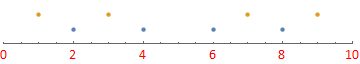
\includegraphics[width=0.5\linewidth]{rnl} 

}

\caption{Conjuntos graficados}\label{fig:rnl1}
\end{figure}

\subsection{Rango}\label{rango}

El rango es la medida de dispersión más fácil de calcular. Se obtiene
restando el máximo menos el mínimo. La expresión para calcularlo es:

\begin{equation} 
  Rango = max - min
  \label{eq:rg}
\end{equation}

\subsection{Varianza}\label{varianza}

La varianza es el promedio de la diferencia de la media cuadrática. Si
se conocen todos los datos de una población se puede calcular la
varianza poblacional:

\begin{equation} 
  \sigma^2 = \dfrac{\sum_{i=1}^{N}\left(x- \mu \right)^2}{N}
  \label{eq:varp}
\end{equation}

Por otro lado si se conocen los datos de una población se puede calcular
la varianza muestral:

\begin{equation} 
  s^2 = \dfrac{\sum_{i=1}^{n}\left(x- \bar{x} \right)^2}{n-1}
  \label{eq:varm}
\end{equation}

\subsection{Desviación}\label{desviacion}

La desviación es la raíz cuadrada de la varianza, en las fórmulas
\eqref{eq:desp} y \eqref{eq:desm} se muestran las expresiones para calcular
la desviación poblacional y muestral respectivamente.

\begin{equation} 
  \sigma = \sqrt{\dfrac{\sum_{i=1}^{N}\left(x- \mu \right)^2}{N}}
  \label{eq:desp}
\end{equation}

\begin{equation} 
  s = \sqrt{\dfrac{\sum_{i=1}^{n}\left(x- \bar{x} \right)^2}{n-1}}
  \label{eq:desm}
\end{equation}

\subsection{Medidas de dispersión en
R}\label{medidas-de-dispersion-en-r}

Es necesario saber que R defecto no tiene una función para calcular el
rango sin embargo para calcular el rango vamos a usar
\texttt{max()\ -\ min()}, y que además por defecto R tiene una función
para calcular la varianza muestral (\texttt{var()}) y otra para calcular
la desviación muestral \texttt{sd()}, si se desea obtener la varianza y
la desviación poblacional existen por lo menos 3 soluciones:

\begin{itemize}
\tightlist
\item
  Se puede multiplicar la varianza muestral por \(\dfrac{n-1}{n}\) para
  obtener la varianza poblacional y la desviación muestral por
  \(\sqrt{\dfrac{n-1}{n}}\) para obtener la desviación poblacional.
\item
  Se puede multiplicar la varianza muestral por \(\dfrac{n-1}{n}\) para
  obtener la varianza poblacional y a ese resultado extraer la raíz
  cuadrada para obtener la desviación poblacional.
\item
  Crear funciones propias que calculen la varianza y la desviación
  muestral.
\end{itemize}

Vamos a trabajar con la segunda solución que es simplemente una mejora
de la primera solución, la tercera solución es avanzada y será abordada
más adelante.

A manera de ejemplo vamos a calcular las medidas de dispersión de los
activos en millones de dólares de la base \texttt{cap2\_big4\_size.csv}.
Se calculan la varianza y la desviación poblacional aunque, a menos de
que tengamos todos los datos (población), siempre en el análisis
estadístico de datos se calcula la varianza y la desviación muestral.

\begin{Shaded}
\begin{Highlighting}[]
\NormalTok{big4size }\OperatorTok
\StringTok{  }\KeywordTok{summarise}\NormalTok{(}\DataTypeTok{RANGO.ACTIVOS =} \KeywordTok{max}\NormalTok{(ACTIVOS}\OperatorTok{/}\DecValTok{1000000}\NormalTok{)}\OperatorTok{-}\KeywordTok{min}\NormalTok{(ACTIVOS}\OperatorTok{/}\DecValTok{1000000}\NormalTok{),}
            \DataTypeTok{VARM.ACTIVOS =} \KeywordTok{var}\NormalTok{(ACTIVOS}\OperatorTok{/}\DecValTok{1000000}\NormalTok{),}
            \DataTypeTok{DESVM.ACTIVOS =} \KeywordTok{sd}\NormalTok{(ACTIVOS}\OperatorTok{/}\DecValTok{1000000}\NormalTok{),}
            \DataTypeTok{n=}\KeywordTok{n}\NormalTok{()}
\NormalTok{            ) }\OperatorTok
\StringTok{  }\KeywordTok{mutate}\NormalTok{(}\DataTypeTok{VARP.ACTIVOS =}\NormalTok{ VARM.ACTIVOS}\OperatorTok{*}\NormalTok{((n}\OperatorTok{-}\DecValTok{1}\NormalTok{)}\OperatorTok{/}\NormalTok{n),}
         \DataTypeTok{DESVP.ACTIVOS =} \KeywordTok{sqrt}\NormalTok{(VARP.ACTIVOS)) }\OperatorTok
\StringTok{  }\KeywordTok{select}\NormalTok{(RANGO.ACTIVOS, VARM.ACTIVOS, DESVM.ACTIVOS, VARP.ACTIVOS, DESVP.ACTIVOS)}
\end{Highlighting}
\end{Shaded}

\begin{verbatim}
##   RANGO.ACTIVOS VARM.ACTIVOS DESVM.ACTIVOS VARP.ACTIVOS DESVP.ACTIVOS
## 1      1341.989     11327.34        106.43     11322.31      106.4064
\end{verbatim}

\section{Tablas de frecuencia}\label{tablas-de-frecuencia}

Una tabla de frecuencia es una forma de describir los datos de forma
resumida, las tablas de frecuencia pueden construirse para variables
cualitativas y para variables cuantitativas.

\subsection{Variables Cualitativas}\label{variables-cualitativas}

Para las variables cualitativas una tabla de frecuencia basicámente
tiene tres columnas: ``Categoría'', ``Frecuencia'', ``Porcentaje''. Para
aprender a realizar tablas de frecuencia para variables cualitativas,
trabajaremos con el conjunto de datos \texttt{audit\_bolsa}, Este
conjunto de datos tiene información sobre las empresas que cotizan en la
Bolsa de Valores de Guayaquil, se elaborará una tabla de frecuencias de
las firmas auditoras que han trabajado para estas empresas. La variable
en la que se almacena esta información es la variable \texttt{FIRMA}. La
tabla de frecuencia se elabora usando el paquete \texttt{dplyr}. El
comando \texttt{mutate(\ )} sirve para crear nuevas columnas, en este
caso se crea la columna porcentaje.

\begin{Shaded}
\begin{Highlighting}[]
\KeywordTok{setwd}\NormalTok{(}\StringTok{"C:/Users/onava_000/OneDrive/libro_mc/estadistica"}\NormalTok{)}
\NormalTok{audit_bolsa <-}\StringTok{ }\KeywordTok{read.csv}\NormalTok{(}\StringTok{"audit_bolsa.csv"}\NormalTok{,}\DataTypeTok{header=}\OtherTok{TRUE}\NormalTok{,}\DataTypeTok{sep=}\StringTok{";"}\NormalTok{,}\DataTypeTok{dec=}\StringTok{","}\NormalTok{)}

\NormalTok{tabla_firma <-}\StringTok{ }\NormalTok{audit_bolsa }\OperatorTok
\StringTok{  }\KeywordTok{group_by}\NormalTok{(FIRMA) }\OperatorTok
\StringTok{  }\KeywordTok{summarise}\NormalTok{(}\DataTypeTok{Frecuencia=}\KeywordTok{n}\NormalTok{()) }\OperatorTok
\StringTok{  }\KeywordTok{mutate}\NormalTok{(}\DataTypeTok{Porcentaje =} \KeywordTok{round}\NormalTok{(}\DecValTok{100}\OperatorTok{*}\NormalTok{Frecuencia}\OperatorTok{/}\KeywordTok{sum}\NormalTok{(Frecuencia),}\DecValTok{2}\NormalTok{)}
\NormalTok{         ) }\OperatorTok
\StringTok{  }\KeywordTok{arrange}\NormalTok{(}\KeywordTok{desc}\NormalTok{(Porcentaje))}
 \KeywordTok{print}\NormalTok{(tabla_firma)}
\end{Highlighting}
\end{Shaded}

\begin{verbatim}
## # A tibble: 15 x 3
##    FIRMA                               Frecuencia Porcentaje
##    <fct>                                    <int>      <dbl>
##  1 DELOITTE                                   103      48.6 
##  2 MOORE STEPHENS                              29      13.7 
##  3 PWC PRICE WATER HOUSE COOPERS               24      11.3 
##  4 HANSEN HOLM & CO. CIA. LTDA.                15       7.08
##  5 KPMG                                        13       6.13
##  6 ERNST & YOUNG                                7       3.3 
##  7 BDO                                          6       2.83
##  8 ALTAMIRANO HIDALGO MARIO ROBERTO             3       1.42
##  9 KRESTON                                      3       1.42
## 10 PKF                                          3       1.42
## 11 BATALLAS & BATALLAS                          2       0.94
## 12 ASE + ASESORANDO MAS                         1       0.47
## 13 CONSULTORES MORAN CEDILLO CIA. LTDA          1       0.47
## 14 HERRERA CHANG 6 ASOCIADOS                    1       0.47
## 15 NGV                                          1       0.47
\end{verbatim}

\label{tab:tabla2}Tabla de Frecuencia de Firmas Auditoras

FIRMA

Frecuencia

Porcentaje

DELOITTE

103

48.58

MOORE STEPHENS

29

13.68

PWC PRICE WATER HOUSE COOPERS

24

11.32

HANSEN HOLM \& CO. CIA. LTDA.

15

7.08

KPMG

13

6.13

ERNST \& YOUNG

7

3.30

BDO

6

2.83

ALTAMIRANO HIDALGO MARIO ROBERTO

3

1.42

KRESTON

3

1.42

PKF

3

1.42

BATALLAS \& BATALLAS

2

0.94

ASE + ASESORANDO MAS

1

0.47

CONSULTORES MORAN CEDILLO CIA. LTDA

1

0.47

HERRERA CHANG 6 ASOCIADOS

1

0.47

NGV

1

0.47

En la tabla \ref{tab:tabla2} se aprecia el resultado obtenido y
formateado para ser publicado. El resultado de R, puede ser exportado a
un archivo Excel con la finalidad de luego tomar esa tabla y llevarla a
un documento donde se presentará toda la información analizada. Para
exportar la información a un archivo excel se puede trabajar con el
paquete \texttt{xlsx}. Para exportar los resultados a Excel se puede
proceder de la siguiente forma.

\begin{enumerate}
\def\labelenumi{\arabic{enumi}.}
\tightlist
\item
  Cargar el paquete \texttt{xlsx}.
\item
  Convertir el resultado a un \texttt{data\ frame} utilizando la función
  \texttt{as.data.frame()}
\item
  Exportar el resultado con la función \texttt{write.xlsx()} cuya
  estructura básica es \texttt{write.xlsx(datos,\ "archivo.xlsx")}, si
  se desea consultar más detalles de la función se puede escribir
  \texttt{?write.xlsx}.
\end{enumerate}

El resultado de esta operación será un archivo de excel guardado en
nuestro directorio de trabajo.

\begin{Shaded}
\begin{Highlighting}[]
\KeywordTok{library}\NormalTok{(xlsx)}
\NormalTok{tabla_firma =}\StringTok{ }\KeywordTok{as.data.frame}\NormalTok{(tabla_firma)}
\KeywordTok{write.xlsx}\NormalTok{(tabla_firma, }\StringTok{"tablas.xlsx"}\NormalTok{, }\DataTypeTok{sheetName =} \StringTok{"firmas"}\NormalTok{, }\DataTypeTok{row.names =} \OtherTok{FALSE}\NormalTok{)}
\end{Highlighting}
\end{Shaded}

La opción \texttt{sheetname\ =\ "firmas"} crea dentro del libro
\texttt{tablas.xlsx} una hoja de cálculo llamada \texttt{firmas}. La
opción \texttt{row.names\ =\ FALSE} hace que en el archivo final no se
graben los números de cada fila.

Nota: es importante tener fijado el directorio de trabajo, como se
explicó en la sección \ref{primerR}.

\subsection{Variables Cuantitativas}\label{variables-cuantitativas}

Una tabla de frecuencias para variables cualitativas tiene 6 columnas:

\begin{enumerate}
\def\labelenumi{\arabic{enumi}.}
\tightlist
\item
  Clase: una clase es un intervalo del tipo
  \(\left[ menor, mayor \right)\)
\item
  Marca de Clase: es un valor igual al promedio de los dos extremos de
  la clase.
\item
  Frecuencia: la frecuencia es igual al número de valores de la variable
  que están dentro del intervalo.
\item
  Frecuencia relativa: la frecuencia relativa se la calcula como la
  frecuencia dividida para el total de valores de la variable.
\item
  Frecuencia acumulada: se la calcula sumando las frecuencias desde la
  primera clase hasta la clase en consideración.
\item
  Frecuencia Relativa acumulada: se la calcula como la frecuencia
  acumulada pero para las frecuencias relativas.
\end{enumerate}

Una de las ventajas de usar R es que se pueden crear funciones para cada
necesidad que el investigador tenga, en este caso el código que se
muestra sirve para hacer tablas de frecuencia de cualquier variable
cuantitativa. A manera de ejemplo se hará la tabla de frecuencia de la
variable \texttt{VTAS} en millones de dólares, del conjunto de datos
trabajado en la sección \ref{primerR}.

\begin{Shaded}
\begin{Highlighting}[]
\KeywordTok{library}\NormalTok{(agricolae)}
\KeywordTok{library}\NormalTok{(dplyr)}

\NormalTok{h2<-}\KeywordTok{with}\NormalTok{(big4size,}\KeywordTok{graph.freq}\NormalTok{(VTAS}\OperatorTok{/}\DecValTok{1000000}\NormalTok{,}\DataTypeTok{plot=}\OtherTok{FALSE}\NormalTok{));}

\NormalTok{h2 =}\StringTok{ }\KeywordTok{table.freq}\NormalTok{(h2)}

\NormalTok{h3 <-}\StringTok{ }\NormalTok{h2 }\OperatorTok
\StringTok{  }\KeywordTok{mutate}\NormalTok{(}\DataTypeTok{Clase =} \KeywordTok{paste}\NormalTok{(}\StringTok{"["}\NormalTok{,Lower,}\StringTok{","}\NormalTok{,Upper,}\StringTok{")"}\NormalTok{),    }
        \StringTok{"Marca de Clase"}\NormalTok{  =}\StringTok{  }\NormalTok{Main,}
        \DataTypeTok{Frec. =}\NormalTok{ Frequency,}
        \StringTok{"Frec. Rel."}\NormalTok{ =}\StringTok{ }\NormalTok{Percentage,}
        \StringTok{"Frec. Acu."}\NormalTok{ =}\StringTok{ }\NormalTok{CF,}
        \StringTok{"Rel. Acu."}\NormalTok{ =}\StringTok{ }\NormalTok{CPF )  }\OperatorTok
\StringTok{  }\KeywordTok{select}\NormalTok{(}\OperatorTok{-}\KeywordTok{c}\NormalTok{(}\DecValTok{1}\OperatorTok{:}\DecValTok{7}\NormalTok{))}
\end{Highlighting}
\end{Shaded}

\label{tab:tabla3}Tabla de Frecuencia de las Ventas

Clase

Marca de Clase

Frec.

Frec. Rel.

Frec. Acu.

Rel. Acu.

{[} 0 , 165.76 )

82.88

2099

93.0

2099

93.0

{[} 165.76 , 331.52 )

248.64

83

3.7

2182

96.7

{[} 331.52 , 497.28 )

414.40

35

1.6

2217

98.3

{[} 497.28 , 663.04 )

580.16

17

0.8

2234

99.0

{[} 663.04 , 828.8 )

745.92

0

0.0

2234

99.0

{[} 828.8 , 994.56 )

911.68

7

0.3

2241

99.3

{[} 994.56 , 1160.32 )

1077.44

12

0.5

2253

99.9

{[} 1160.32 , 1326.08 )

1243.20

0

0.0

2253

99.9

{[} 1326.08 , 1491.84 )

1408.96

0

0.0

2253

99.9

{[} 1491.84 , 1657.6 )

1574.72

0

0.0

2253

99.9

{[} 1657.6 , 1823.36 )

1740.48

2

0.1

2255

100.0

{[} 1823.36 , 1989.12 )

1906.24

1

0.0

2256

100.0

De la tabla \ref{tab:tabla3} se obsserva que el \(93\%\) de las empresas
realiza ventas entre 0 y \(165.76\) millones. El \(99\%\) de las
empresas es decir \(2234\) tiene ventas menores a \(663.04\) millones de
dólares, esto se lo puede ver en la columna de frecuencias acumuladas
relativas. Además, solo una empresa tiene ventas entre \(1823.36\) y
\(1989.12\) millones. Finalmente vamos a exportar la tabla de frecuencia
en el archivo \texttt{tablas.xlsx}. La opción \texttt{append\ =\ TRUE}
sirve para añadir una nueva hoja de cálculo al libro.

\begin{Shaded}
\begin{Highlighting}[]
\KeywordTok{library}\NormalTok{(xlsx)}
\NormalTok{h3 =}\StringTok{ }\KeywordTok{as.data.frame}\NormalTok{(h3)}
\KeywordTok{write.xlsx}\NormalTok{(h3, }\StringTok{"tablas.xlsx"}\NormalTok{, }\DataTypeTok{sheetName =} \StringTok{"frec_ventas"}\NormalTok{, }\DataTypeTok{row.names =} \OtherTok{FALSE}\NormalTok{,}\DataTypeTok{append=}\OtherTok{TRUE}\NormalTok{)}
\end{Highlighting}
\end{Shaded}

\section{Tablas de Contingencia}\label{tablas-de-contingencia}

Una tabla de contingencia es una forma útil para examinar relaciones
entre dos variables categóricas. Los valores en las celdas de una tabla
de contingencia pueden ser de frecuencia absoluta o frecuencia relativa.

Para ejemplificar la construcción de una tabla de contingencia vamos a
trabajar con el archivo \texttt{Ranking2018Guayas.csv} este archivo
contiene información sobre una muestra de 162 empresas de la provincia
del Guayas. Se analizará la relación entre la ciudad y el tamaño de las
empresas.

\begin{Shaded}
\begin{Highlighting}[]
\KeywordTok{setwd}\NormalTok{(}\StringTok{"C:/Users/onava_000/OneDrive/libro_mc/estadistica"}\NormalTok{)}
\NormalTok{rank2018 =}\StringTok{ }\KeywordTok{read.csv}\NormalTok{(}\StringTok{"Ranking2018Guayas.csv"}\NormalTok{,}\DataTypeTok{header=}\OtherTok{TRUE}\NormalTok{, }\DataTypeTok{sep=}\StringTok{";"}\NormalTok{)}


\NormalTok{ciudad.tama =}\StringTok{ }\NormalTok{rank2018 }\OperatorTok\StringTok{ }
\StringTok{  }\KeywordTok{group_by}\NormalTok{(CIUDAD, TAMAÑO)}\OperatorTok
\StringTok{  }\KeywordTok{summarise}\NormalTok{(}\DataTypeTok{n=}\KeywordTok{n}\NormalTok{())}\OperatorTok
\StringTok{  }\KeywordTok{spread}\NormalTok{(TAMAÑO, n) }\OperatorTok
\StringTok{  }\KeywordTok{replace}\NormalTok{(., }\KeywordTok{is.na}\NormalTok{(.), }\DecValTok{0}\NormalTok{)}
\end{Highlighting}
\end{Shaded}

\label{tab:tabla4}Tabla de Contingencia de las empresas clasificadas por
tamaño y ciudad

CIUDAD

MEDIANA

MICROEMPRESA

PEQUEÑA

DAULE

1

1

0

ELOY ALFARO

0

2

0

GUAYAQUIL

2

117

28

MILAGRO

0

2

0

NARANJITO

0

4

0

SAMBORONDÓN

0

0

1

SANTA LUCIA

0

1

0

VELASCO IBARRA

0

1

1

En la tabla \ref{tab:tabla4} se observa que de las 162 empresas 117 son
microempresas y de la ciudad de Guayaquil, de la ciudad de Samborondón
se ha tomada una empresa pequeña. Esta información, como se mencionó
antes, puede también ser mostrada en porcentajes. En la tabla
\ref{tab:tabla5} se observa la tabla de contingencia con los
porcentajes.

\begin{Shaded}
\begin{Highlighting}[]
\NormalTok{ciudad.tama.porc =}\StringTok{ }\NormalTok{rank2018 }\OperatorTok\StringTok{ }
\StringTok{  }\KeywordTok{group_by}\NormalTok{(CIUDAD, TAMAÑO)}\OperatorTok
\StringTok{  }\KeywordTok{summarise}\NormalTok{(}\DataTypeTok{Porc =} \KeywordTok{round}\NormalTok{(}\DecValTok{100}\OperatorTok{*}\KeywordTok{n}\NormalTok{()}\OperatorTok{/}\KeywordTok{nrow}\NormalTok{(rank2018),}\DecValTok{2}\NormalTok{)) }\OperatorTok
\StringTok{  }\KeywordTok{spread}\NormalTok{(TAMAÑO, Porc) }\OperatorTok
\StringTok{  }\KeywordTok{replace}\NormalTok{(., }\KeywordTok{is.na}\NormalTok{(.), }\DecValTok{0}\NormalTok{)}
\end{Highlighting}
\end{Shaded}

\label{tab:tabla5}Tabla de Contingencia de las empresas clasificadas por
tamaño y ciudad

CIUDAD

MEDIANA

MICROEMPRESA

PEQUEÑA

DAULE

0.62

0.62

0.00

ELOY ALFARO

0.00

1.24

0.00

GUAYAQUIL

1.24

72.67

17.39

MILAGRO

0.00

1.24

0.00

NARANJITO

0.00

2.48

0.00

SAMBORONDÓN

0.00

0.00

0.62

SANTA LUCIA

0.00

0.62

0.00

VELASCO IBARRA

0.00

0.62

0.62

\section{Gráficos y Visualización}\label{graficos-y-visualizacion}

Para realizar gráficas R tiene algunos paquetes disponibles, sin embargo
en este texto trabajaremos con el paquete \texttt{ggplot2}. Este paquete
está basada en la gramática de los gráficos \citep{wilkinson2005}.

\subsection{Histogramas}\label{histogramas}

Los histogramas se utilizan para variables continuas. Un histograma es
un gráfico de la distribución de frecuencia de una variable, en el eje
vertical se representa la frecuencia (absoluta o relativa) y en el eje
horizontal los rangos de los valores.

En la figura \ref{fig:figura1} se muestra el histograma de la variable
ventas en millones de dólares del archivo \emph{cap2\_big4\_size.csv} ya
descrito en la sección \ref{primerR}, este primer histograma ha sido
configurado para presentar 12 barras, que las barras sean de color azul
con un contorno rojo. Antes de abordar los detalles mencionados
discutiremos brevemente el funcionamiento de la gramática de
\texttt{ggplot2}, una gráfica realizada en \texttt{ggplot2} empieza por
\texttt{ggplot(data,\ aes())} dentro de \texttt{aes()} se indica las
variables que van a intervenir en la gráfica, Luego se añade la
\texttt{geom} con la que se va a trabajar en este caso se escogió
\texttt{geom\_histogram()} puesto que se desea realizar un histograma.
Como se indicó anteriormente se configuró el histograma con 12 barras
(\texttt{bins=12}), la opción \texttt{color="red"} permite que el
contorno de las barrras sea rojo y la opción \texttt{fill="blue"}hace
que las barras sean de color azul.

\begin{Shaded}
\begin{Highlighting}[]
\KeywordTok{library}\NormalTok{(ggplot2)}

\KeywordTok{ggplot}\NormalTok{(big4size, }\KeywordTok{aes}\NormalTok{(}\DataTypeTok{x=}\NormalTok{ VTAS}\OperatorTok{/}\DecValTok{1000000}\NormalTok{)) }\OperatorTok{+}\StringTok{ }
\StringTok{  }\KeywordTok{geom_histogram}\NormalTok{(}\DataTypeTok{bins=}\DecValTok{12}\NormalTok{, }\DataTypeTok{color=} \StringTok{"red"}\NormalTok{, }\DataTypeTok{fill=}\StringTok{"blue"}\NormalTok{ )}
\end{Highlighting}
\end{Shaded}

\begin{figure}
\centering
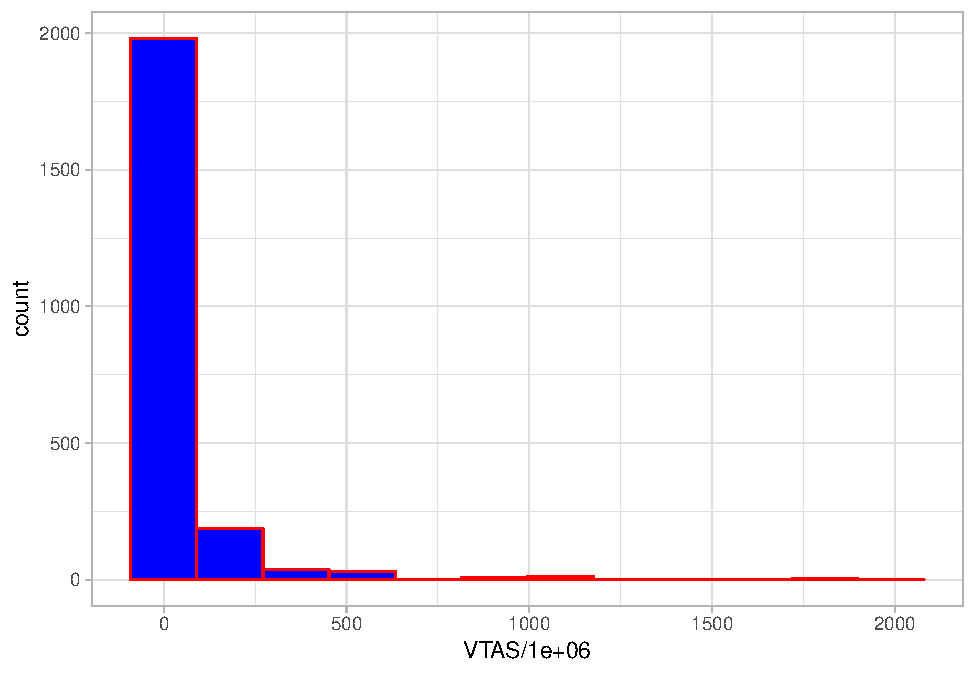
\includegraphics{estadistica_files/figure-latex/figura1-1.pdf}
\caption{\label{fig:figura1}Histograma de las Ventas}
\end{figure}

Para configurar las etiquetas de los ejes podemos añadir las opciones
\texttt{xlab(\ )} y \texttt{ylab(\ )}. En la figura \ref{fig:figura2} se
aprecia el histograma con las etiquetas de los ejes añadidos.

\begin{Shaded}
\begin{Highlighting}[]
\KeywordTok{library}\NormalTok{(ggplot2)}

\KeywordTok{ggplot}\NormalTok{(big4size, }\KeywordTok{aes}\NormalTok{(}\DataTypeTok{x=}\NormalTok{ VTAS}\OperatorTok{/}\DecValTok{1000000}\NormalTok{)) }\OperatorTok{+}\StringTok{ }
\StringTok{  }\KeywordTok{geom_histogram}\NormalTok{(}\DataTypeTok{bins=}\DecValTok{12}\NormalTok{, }\DataTypeTok{color=} \StringTok{"red"}\NormalTok{,  }\DataTypeTok{fill=}\StringTok{"blue"}\NormalTok{ ) }\OperatorTok{+}\StringTok{ }
\StringTok{  }\KeywordTok{xlab}\NormalTok{(}\StringTok{"Ventas en Millones de Dólares") + ylab("}\NormalTok{Frecuencia}\StringTok{")}
\end{Highlighting}
\end{Shaded}

\begin{figure}
\centering
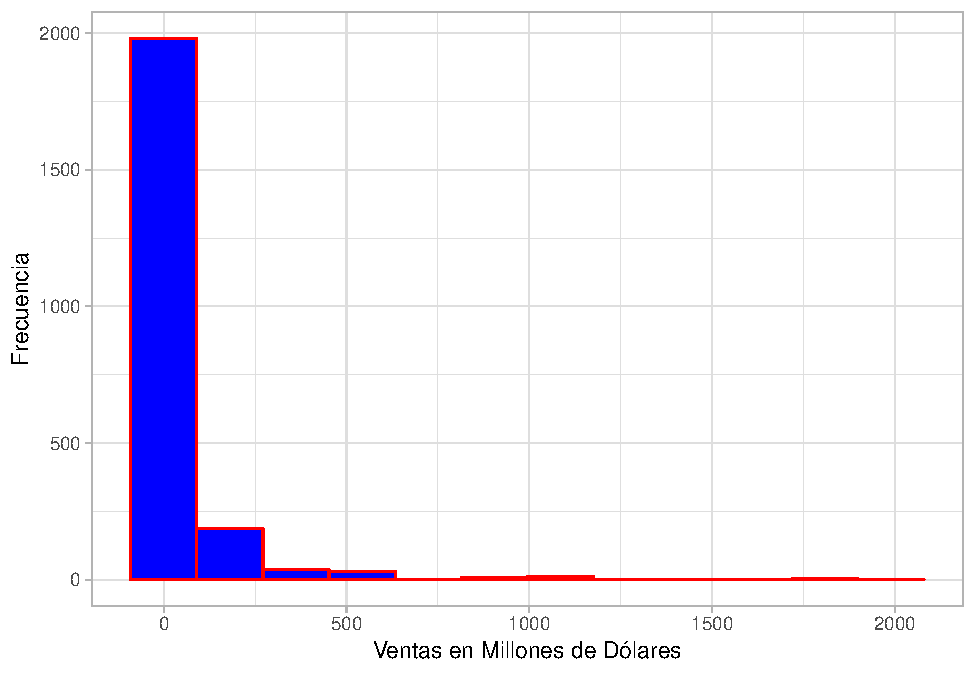
\includegraphics{estadistica_files/figure-latex/figura2-1.pdf}
\caption{\label{fig:figura2}Histograma de las Ventas con Etiquetas en los
Ejes}
\end{figure}

Usando el archivo \texttt{Ranking2018Guayas.csv}, vamos ahora a hacer el
histograma de las ventas en miles de acuerdo al tamaño de la empresa. En
la figura \ref{fig:figura3} se observa el histograma.

Para elaborar este histograma se tomaron en cuenta varias cosas, lo
primero se estimaron los valores máximo y mínimo de la variable.

\begin{Shaded}
\begin{Highlighting}[]
\KeywordTok{min}\NormalTok{(rank2018}\OperatorTok{$}\NormalTok{VENTAS}\OperatorTok{/}\DecValTok{1000}\NormalTok{)}
\NormalTok{## [1] 0}
\KeywordTok{max}\NormalTok{(rank2018}\OperatorTok{$}\NormalTok{VENTAS}\OperatorTok{/}\DecValTok{1000}\NormalTok{)}
\NormalTok{## [1] 1347.729}
\end{Highlighting}
\end{Shaded}

Los valores obtenidos para el máximo y el mínimo fueron \(0\) y \(1348\)
respectivamente, por esta razón se decidió crear 10 clases y cada clase
con una longitud de 150. Adicionalmente para obtener un gráfico
agradable a la vista se cambia la orientación de las marcas de
\(0^\circ\) a \(90^\circ\) en el eje \(x\) con la instrucción
\texttt{theme(axis.text.x\ =\ element\_text(angle\ =\ 90,\ hjust\ =\ 1))}.

\begin{Shaded}
\begin{Highlighting}[]
\KeywordTok{ggplot}\NormalTok{(rank2018, }\KeywordTok{aes}\NormalTok{(}\DataTypeTok{x=}\NormalTok{VENTAS}\OperatorTok{/}\DecValTok{1000}\NormalTok{, }\DataTypeTok{fill=}\NormalTok{TAMAÑO)) }\OperatorTok{+}\StringTok{ }
\StringTok{  }\KeywordTok{geom_histogram}\NormalTok{(}\DataTypeTok{alpha=}\FloatTok{0.3}\NormalTok{, }\DataTypeTok{color=}\StringTok{"black"}\NormalTok{,}\DataTypeTok{bins=}\DecValTok{10}\NormalTok{, }\DataTypeTok{binwidth =} \DecValTok{150}\NormalTok{) }\OperatorTok{+}
\StringTok{  }\KeywordTok{scale_x_continuous}\NormalTok{(}\DataTypeTok{breaks =} \KeywordTok{seq}\NormalTok{(}\DecValTok{0}\NormalTok{,}\DecValTok{1350}\NormalTok{,}\DecValTok{150}\NormalTok{)) }\OperatorTok{+}
\StringTok{  }\KeywordTok{theme}\NormalTok{(}\DataTypeTok{axis.text.x =} \KeywordTok{element_text}\NormalTok{(}\DataTypeTok{angle =} \DecValTok{90}\NormalTok{, }\DataTypeTok{hjust =} \DecValTok{1}\NormalTok{)) }\OperatorTok{+}
\StringTok{  }\KeywordTok{xlab}\NormalTok{(}\StringTok{"Ventas en Miles"}\NormalTok{) }\OperatorTok{+}\StringTok{ }\KeywordTok{ylab}\NormalTok{(}\StringTok{"Frecuencia"}\NormalTok{) }
\end{Highlighting}
\end{Shaded}

\begin{figure}
\centering
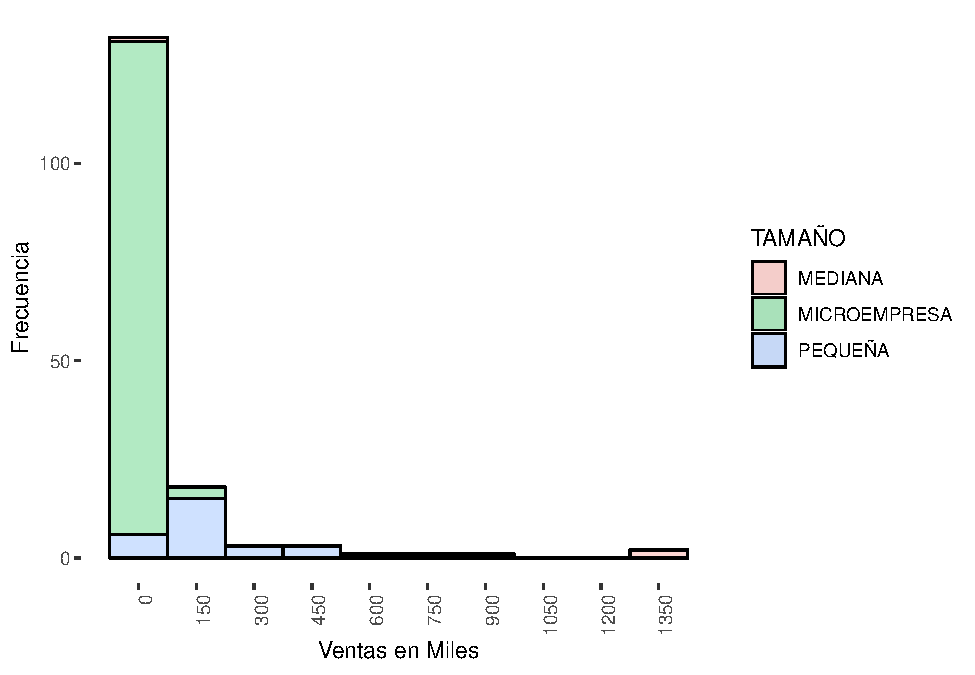
\includegraphics{estadistica_files/figure-latex/figura3-1.pdf}
\caption{\label{fig:figura3}Histograma de las Ventas de Acuerdo al Tamaño de
la empresa}
\end{figure}

Se puede observar en la \ref{fig:figura3} que algunas empresas medianas
tienen mayores ventas que el resto de empresas. Una mejor forma de
comparar la distribución de una variable de acuerdo a otra variable es
usar los diagramas de caja que serán discutidos en profundidad en la
sección \ref{boxes}.

\subsection{Diagramas de Caja y valores atípicos}\label{boxes}

En la \ref{fig:figura3} se pretendía mostrar la distribución de las
ventas de acuerdo al tamaño de la empresa. Sin embargo el histograma no
mostraba claramente la distribución de acuerdo al tamaño de la empresa.
una alternativa es usar un diagrama de caja.

Un diagrama de caja está formado por 5 valores que lo resumen, estos 5
valores se muestran en la figura \ref{fig:caja1}. La distancia entre el
primer y el tercer cuartil se la conoce como rango intercuartílico (IQR,
por sus siglas en inglés). El límite superior es igual al tercer cuartil
más 1.5 veces el rango intercuartílico, valores mayores a esta cantidad
se consideran valores atípicos. Mientras que el límite inferior es igual
al primer cuartil menos 1.5 veces el rango intercuartílico y valores
menores a esta cantidad se consideran valores atípicos.

\begin{equation} 
  IQR = Q_3 - Q_1
  \label{eq:iqr}
\end{equation}

\begin{equation} 
  LS = Q_3 + 1.5IQR
  \label{eq:ls}
\end{equation}

\begin{equation} 
  LI = Q_1 - 1.5IQR
  \label{eq:li}
\end{equation}

\begin{figure}[h]

{\centering 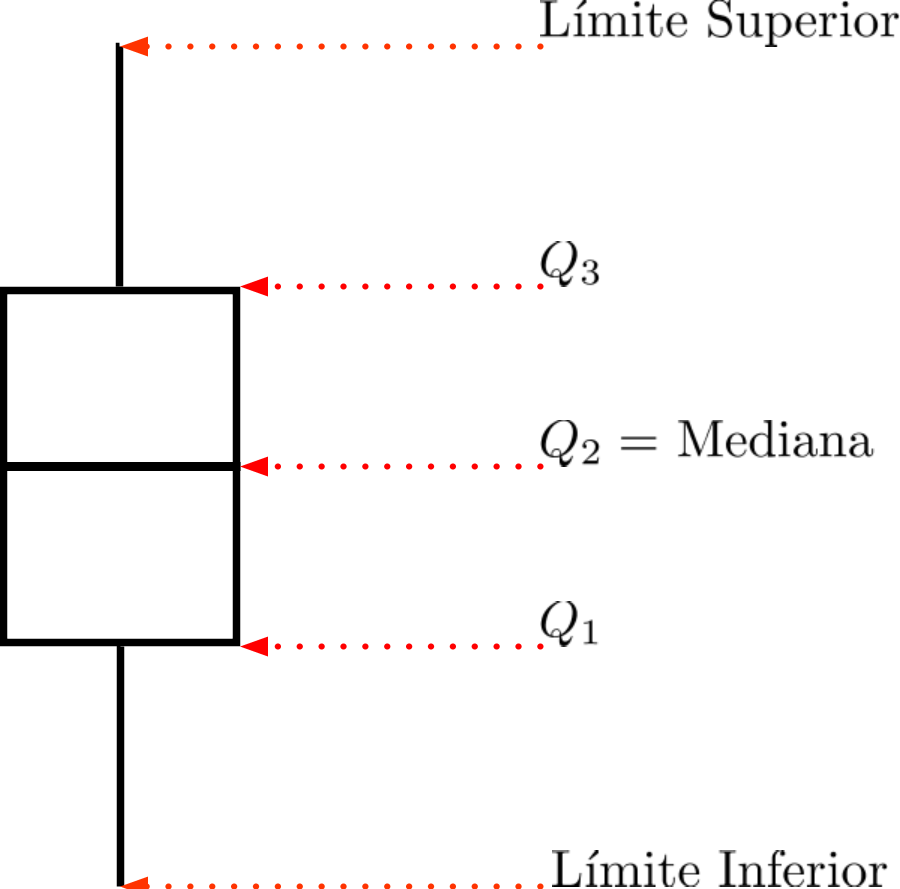
\includegraphics[width=0.4\linewidth]{boxplot3} 

}

\caption{Partes de un Diagrama de Caja}\label{fig:caja1}
\end{figure}

En la figura \ref{fig:figura4} se observan los diagramas de caja de las
ventas según el tamaño de la empresa. Se puede notar que existen
diferencias entre las ventas de las empresas medianas, las microempresas
y las pequeñas. El \(50\%\) de las empresas medianas vende más de
\(1250000\), mientras que todas las microempresas venden menos de
\(250000\). Las empresas pequeñas que venden más de \(500000\) son
atípicas, mientras que en las empresas medianas no se presentan valores
atípicos.

\begin{Shaded}
\begin{Highlighting}[]
\KeywordTok{ggplot}\NormalTok{(rank2018, }\KeywordTok{aes}\NormalTok{(TAMAÑO, VENTAS}\OperatorTok{/}\DecValTok{1000}\NormalTok{)) }\OperatorTok{+}\StringTok{ }
\StringTok{  }\KeywordTok{geom_boxplot}\NormalTok{() }\OperatorTok{+}\StringTok{ }\KeywordTok{xlab}\NormalTok{(}\StringTok{"Tamaño de las empresas"}\NormalTok{) }\OperatorTok{+}
\StringTok{  }\KeywordTok{ylab}\NormalTok{(}\StringTok{"Ventas en Miles de Dólares")}
\end{Highlighting}
\end{Shaded}

\begin{figure}
\centering
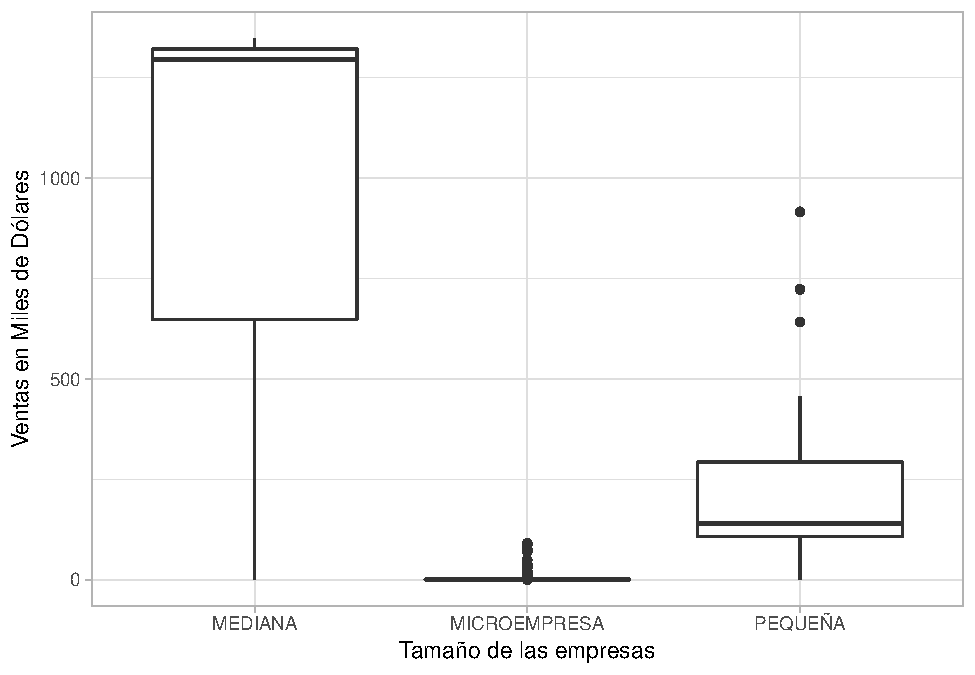
\includegraphics{estadistica_files/figure-latex/figura4-1.pdf}
\caption{\label{fig:figura4}Diagrama de Caja de las Ventas según el Tamaño
de la empresa}
\end{figure}

Si se quisiera analizar con mayor detalle las microempresas se podría
seleccionar solo las empresas con este tamaño y elaborar el diagrama de
caja correspondiente, para lograr esto se utiliza la función
\texttt{subset(df,\ cond)}. donde \texttt{df} corresponde al \emph{data
frame} usado y \emph{cond} a la regla que deben cumplir los datos a ser
analizados.

\begin{Shaded}
\begin{Highlighting}[]
\KeywordTok{ggplot}\NormalTok{(}\KeywordTok{subset}\NormalTok{(rank2018, TAMAÑO }\OperatorTok{==}\StringTok{ "MICROEMPRESA"}\NormalTok{), }\KeywordTok{aes}\NormalTok{(TAMAÑO, VENTAS}\OperatorTok{/}\DecValTok{1000}\NormalTok{)) }\OperatorTok{+}\StringTok{ }
\StringTok{  }\KeywordTok{geom_boxplot}\NormalTok{() }\OperatorTok{+}\StringTok{ }\KeywordTok{xlab}\NormalTok{(}\StringTok{""}\NormalTok{) }\OperatorTok{+}
\StringTok{  }\KeywordTok{ylab}\NormalTok{(}\StringTok{"Ventas en Miles de Dólares")}
\end{Highlighting}
\end{Shaded}

\begin{figure}
\centering
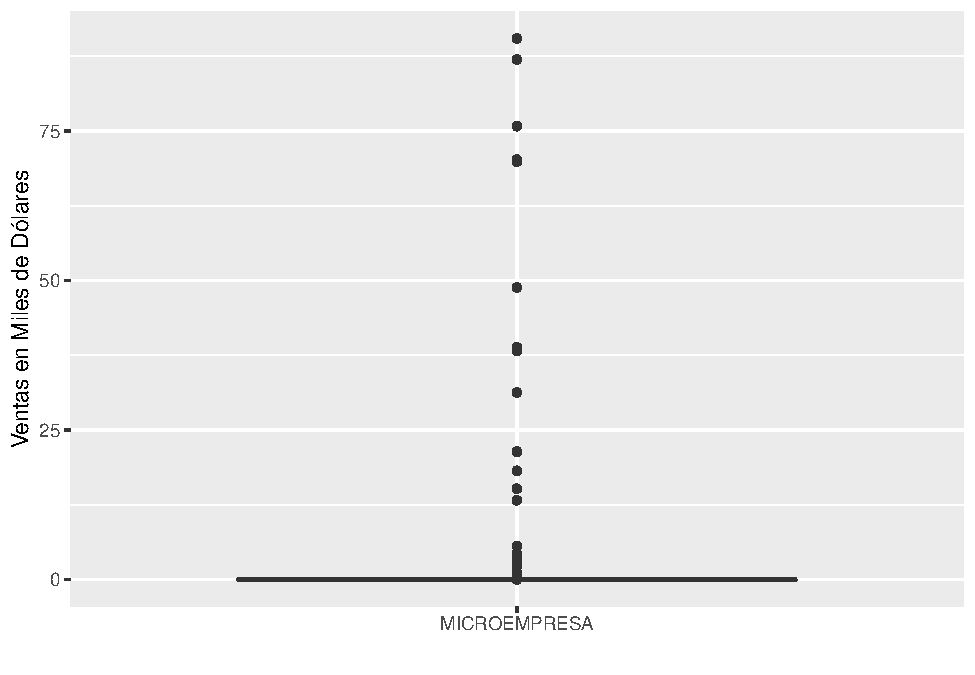
\includegraphics{estadistica_files/figure-latex/figura5-1.pdf}
\caption{\label{fig:figura5}Diagrama de Caja de las Ventas de las
Microempresas}
\end{figure}

\chapter{Intervalos de Confianza y Pruebas de
Hipótesis}\label{intervalos-de-confianza-y-pruebas-de-hipotesis}

En la sección \ref{estypes} se habló de los típos de estadística, la
estadística inferencial consiste de los métodos por medio de los cuales
se puede hacer inferencias o generalizaciones sobre una población. La
inferencia estadística se puede dívidir en dos grandes áreas:
\textbf{estimación} y \textbf{pruebas de hipótesis}.

Imaginemos que se desea estimar el promedio de las ventas en miles de
las empresas que son auditadas por firmas Big Four, sin embargo debemos
recordar que en nuestro conjunto de datos no tenemos a todas las
empresas sino a una muestra de las empresas, por lo que afirmar que el
valor obtenido es el promedio de todas las empresas auditadas por Big
Four es el valor real es muy arriesgado. Sin embargo, podríamos dar un
intervalo en el que posiblemente se encuentre el valor que deseamos
estimar.

Ahora supongamos que usted como investigador quiere probar que el
promedio de las ventas en miles de las empresas que son auditadas por
una Big Four es mayor a las empresas que no son auditadas por una Big
Four. Una primera aproximación para resolver este problema es realizar
una gráfica que le muestre las ventas de acuerdo al tipo de empresa
auditora.

Antes de elaborar el gráfico vamos a crear una nueva variable llamada
\texttt{Big4}en la que si la variable `\texttt{BIG4} es igual a 1 la
variable \texttt{Big4} tomará el valor de Sí, caso contrario tomará el
valor de No.

\begin{Shaded}
\begin{Highlighting}[]
\NormalTok{big4size <-}\StringTok{ }\NormalTok{big4size }\OperatorTok
\StringTok{  }\KeywordTok{mutate}\NormalTok{(}
    \DataTypeTok{Big4 =} \KeywordTok{ifelse}\NormalTok{(BIG4}\OperatorTok{==}\DecValTok{1}\NormalTok{, }\StringTok{"Sí"}\NormalTok{,}\StringTok{"No"}\NormalTok{)}
\NormalTok{  )}
\end{Highlighting}
\end{Shaded}

En las figuras \ref{fig:figura6} y \ref{fig:figura7} se observa el
histograma y el diagrama de caja de las ventas de acuerdo a la firma
auditora. Al observar las gráficas se puede afirmar que evidentemente el
promedio de las ventas de las empresas auditadas por firmas Big Four es
mayor, sin embargo en estadística no se puede confirmar o negar una
afirmación con solo ver un gráfico.

\begin{Shaded}
\begin{Highlighting}[]
\KeywordTok{ggplot}\NormalTok{(big4size, }\KeywordTok{aes}\NormalTok{(}\DataTypeTok{x=}\NormalTok{VTAS}\OperatorTok{/}\DecValTok{1000}\NormalTok{, }\DataTypeTok{fill=}\NormalTok{Big4)) }\OperatorTok{+}\StringTok{ }
\StringTok{  }\KeywordTok{geom_histogram}\NormalTok{(}\DataTypeTok{alpha=}\FloatTok{0.3}\NormalTok{, }\DataTypeTok{color=}\StringTok{"black"}\NormalTok{,}\DataTypeTok{bins=}\DecValTok{10}\NormalTok{, }\DataTypeTok{binwidth =} \DecValTok{200000}\NormalTok{) }\OperatorTok{+}
\StringTok{  }\KeywordTok{scale_x_continuous}\NormalTok{(}\DataTypeTok{breaks =} \KeywordTok{seq}\NormalTok{(}\DecValTok{0}\NormalTok{,}\DecValTok{2000000}\NormalTok{,}\DecValTok{200000}\NormalTok{)) }\OperatorTok{+}
\StringTok{  }\KeywordTok{theme}\NormalTok{(}\DataTypeTok{axis.text.x =} \KeywordTok{element_text}\NormalTok{(}\DataTypeTok{angle =} \DecValTok{90}\NormalTok{, }\DataTypeTok{hjust =} \DecValTok{1}\NormalTok{)) }\OperatorTok{+}
\StringTok{  }\KeywordTok{xlab}\NormalTok{(}\StringTok{"Ventas en Miles"}\NormalTok{) }\OperatorTok{+}\StringTok{ }\KeywordTok{ylab}\NormalTok{(}\StringTok{"Frecuencia"}\NormalTok{) }
\end{Highlighting}
\end{Shaded}

\begin{figure}
\centering
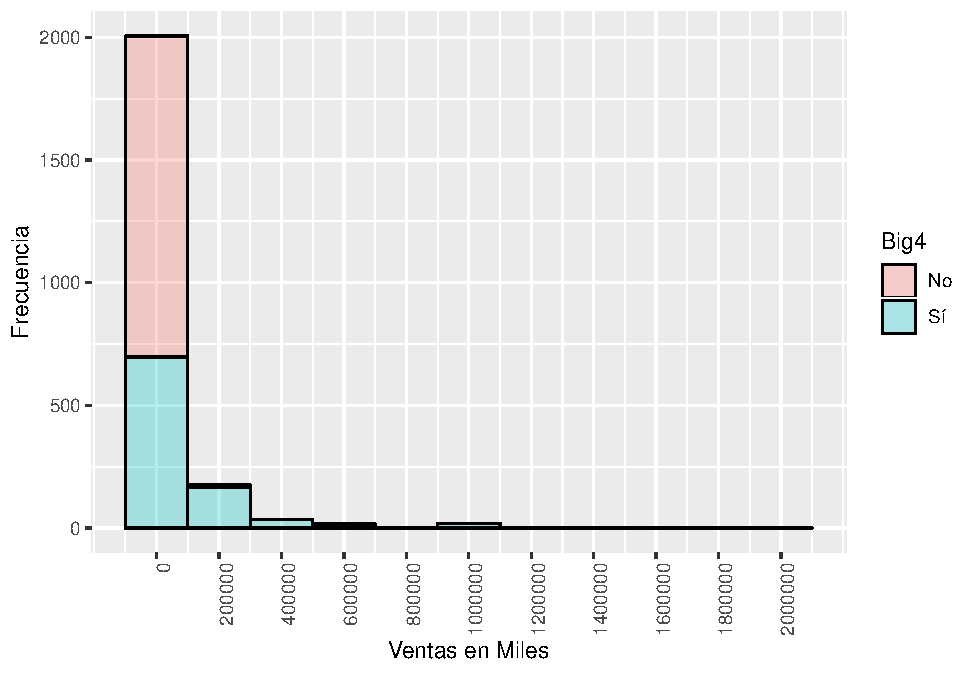
\includegraphics{estadistica_files/figure-latex/figura6-1.pdf}
\caption{\label{fig:figura6}Histograma de las Ventas de Acuerdo al tipo de
Firma Auditora}
\end{figure}

\begin{Shaded}
\begin{Highlighting}[]
\KeywordTok{ggplot}\NormalTok{(big4size, }\KeywordTok{aes}\NormalTok{(Big4, VTAS}\OperatorTok{/}\DecValTok{1000}\NormalTok{)) }\OperatorTok{+}\StringTok{ }
\StringTok{  }\KeywordTok{geom_boxplot}\NormalTok{() }\OperatorTok{+}\StringTok{ }\KeywordTok{xlab}\NormalTok{(}\StringTok{"Tipo de Firma"}\NormalTok{) }\OperatorTok{+}
\StringTok{  }\KeywordTok{ylab}\NormalTok{(}\StringTok{"Ventas en Miles de Dólares")}
\end{Highlighting}
\end{Shaded}

\begin{figure}
\centering
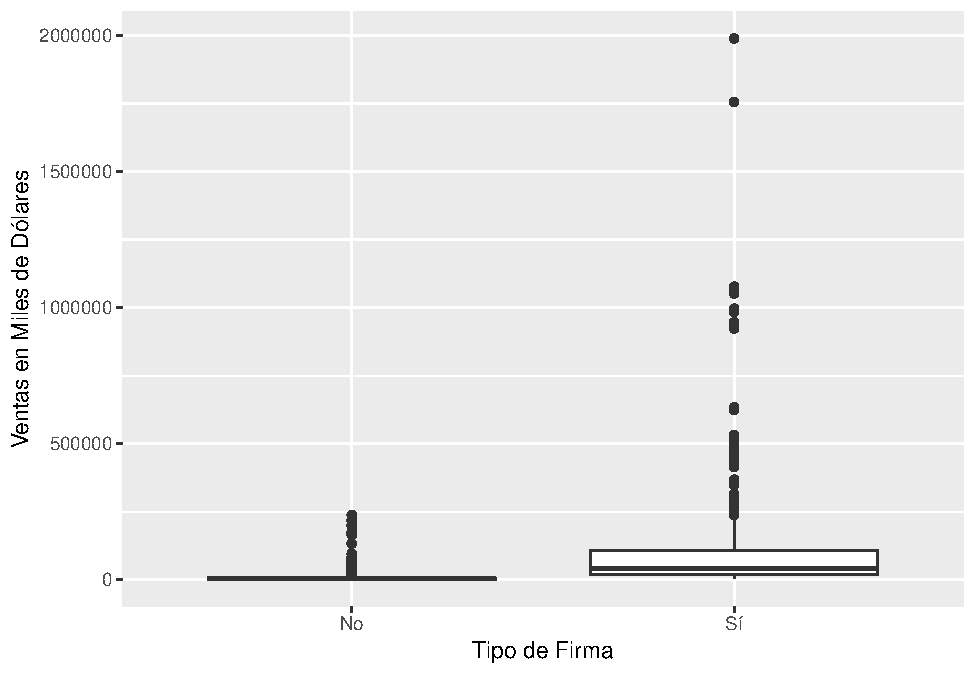
\includegraphics{estadistica_files/figure-latex/figura7-1.pdf}
\caption{\label{fig:figura7}Diagrama de Caja de las Ventas de Acuerdo al
tipo de Firma Auditora}
\end{figure}

Los dos problemas citados serán abordados y resueltos en este capítulo.
El primero en la sección \ref{ic} y el segundo en la sección \ref{ph}.

\section{Intervalos de Confianza}\label{ic}

Un \emph{estimador puntual} de un parámetro \(\theta\) es un número
\(\bar{\theta}\) de un estadístico \(\Theta\) que puede ser considerado
un valor que se aproxima a \(\theta\). Por ejemplo \(\bar{x}\) del
estadístico \(\bar{X}\), calculado de una muestra de tamaño \(n\) es un
estimador puntual del parámetro poblacional \(\mu\). Debido a que un
estimador puntual es un simple número, no da información por si solo
sobre la precisión y la confiabilidad de la estimación.

En cualquier estimación de un parámetro habrá un error asociado, por
ejemplo \(\bar{X}\) no debe estimar \(\mu\) con exactitud, pero se
espera que no esté muy lejos del valor real. Lo que se espera de un
estimador es que sea insesgado y eficiente.

La forma de un intervalo de confianza es:

\begin{equation} 
  \text{Estimador puntual} \pm \text{Margen de Error}
  \label{eq:ic}
\end{equation}

El estimador es el valor calculado a partir de la muestra para el
parámetro desconocido. El \emph{margen de error} es cuán preciso es
nuestro cálculo, basados en la variabilidad del estimador, y de la
confianza que tengamos en que el procedimiento detectará el valor real
del parámetro de la población.

\subsection{Interpretación de un intervalo de
confianza}\label{interpretacion-de-un-intervalo-de-confianza}

Un intervalo de confianza del \(C \%\) indica que si construimos muchos
de esos intervalos, entonces el \(C \%\) de las veces el intervalo
contendrá el valor real del parámetro.

Por ejemplo en la figura \ref{fig:ic} se muestran 100 intervalos
construidos con el \(95 \%\) de confianza para el promedio poblacional,
para construir cada intervalo se tomaron muestras de 100 elementos. Los
intervalos de color celeste son los que contienen el valor real del
parámetro, los intervalos de color rojo son los que no contienen el
valor real del parámetro. El lector puede verificar que \(5\) intervalos
es decir el \(5 \%\) no contiene el valor real del parámetro lo que
implica que el \(95 \%\) de los intervalos sí contiene el valor real del
parámetro.

\begin{figure}[h]

{\centering 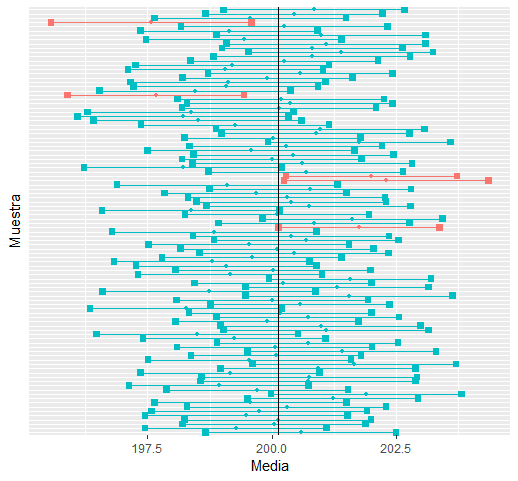
\includegraphics[width=0.7\linewidth]{ic} 

}

\caption{Intervalos de Confianza simulados}\label{fig:ic}
\end{figure}

\subsection{\texorpdfstring{Intervalo de Confianza para la media
\(\mu\)}{Intervalo de Confianza para la media \textbackslash{}mu}}\label{intervalo-de-confianza-para-la-media-mu}

Para construir un intervalo de confianza para \(\mu\) existen dos casos,
el primero es cuando se conoce la desviación poblacional \(\sigma\) y el
segundo cuando no se conoce la desviación poblacional \(\sigma\).El
primer caso es hipotético y puede ser considerado un caso para
ejemplificar el concepto de intervalo de confianza, en la sección
\ref{jt} se explica en detalle por qué consideramos este un caso
hipotético. Para el primer caso usamos la distribución normal y para el
segundo debemos usar otra distribución como lo veremos en la sección
\ref{icsd}.

\subsubsection{\texorpdfstring{Intervalo de confianza para \(\mu\)
cuando se conoce
\(\sigma\)}{Intervalo de confianza para \textbackslash{}mu cuando se conoce \textbackslash{}sigma}}\label{jt}

Si \(\bar{x}\) es la media de una muestra aleatoria de tamaño \(n\) de
una población con desviación conocida \(\sigma\), un intervalo con
\(100\left(1-\alpha\right)\%\) para la media \(\mu\) está dado por:

\begin{equation} 
  \left(\bar{x} - Z_{\frac{\alpha}{2}}\dfrac{\sigma}{\sqrt{n}}, \bar{x} + Z_{\frac{\alpha}{2}}\dfrac{\sigma}{\sqrt{n}}  \right)
  \label{eq:icmusc}
\end{equation}

Donde \(Z_{\frac{\alpha}{2}}\) es el valor correspondiente a una
probabilidad de cola superior de \(\frac{\alpha}{2}\) de la distribución
normal estándar. El valor de \(Z_{\frac{\alpha}{2}}\) que se usa para
construir un intervalo de confianza recibe el nombre de \emph{valor
crítico}.

Para utilizar la ecuación \eqref{eq:icmusc} es necesario conocer el valor
de \(\sigma\). Pero conocer \(\sigma\) implica conocer toodos los
valores de la población. Y si se conocen todos los valores de la
población se puede calcular el valor de la media poblacional que es lo
que nos interesa estimar. En situaciones empresariales y financieras
nunca se conoce la desviación estándar de la población y además las
poblaciones son muy grandes lo que imposibilita poder examinar todos los
valores. En la siguiente sección aprenderemos a abordar esta situación.

\subsubsection{\texorpdfstring{Intervalo de confianza para \(\mu\)
cuando no se conoce
\(\sigma\)}{Intervalo de confianza para \textbackslash{}mu cuando no se conoce \textbackslash{}sigma}}\label{icsd}

Si \(\bar{x}\) es la media de una muestra aleatoria de tamaño \(n\) con
desviación muestral \(s\), un intervalo con
\(100\left(1-\alpha\right)\%\) para la media \(\mu\) está dado por:

\begin{equation} 
  \left(\bar{x} - t_{\frac{\alpha}{2}}\dfrac{s}{\sqrt{n}}, \bar{x} + t_{\frac{\alpha}{2}}\dfrac{s}{\sqrt{n}}  \right)
  \label{eq:icmusd}
\end{equation}

donde \(t_{\dfrac{\alpha}{2}}\) es el valor crítico correspondiente a
una probabilidad de cola superior de \(\dfrac{\alpha}{2}\) de la
distribución \(t\) con \(n-1\) grados de libertad.

\subsection{Intervalo de Confianza para la
proporción}\label{intervalo-de-confianza-para-la-proporcion}

Los dos intervalos de confianza vistos en las secciones anteriores son
usados para variables cuantitativas, también se puede crear intervalos
de confianza para variables categóricas. Por ejemplo, es posible que
queramos estimar la proporción de elementos en una población que poseen
cierta propiedad de interés. El parámetro de la proporción poblacional
lo vamos a representar con la letra griega \(\pi\). El estimador puntual
para \(\pi\) es la proporción muestral \(p=\frac{X}{n}\), donde \(n\) es
el tamaño muestral y \(X\) es el número de elementos de la muestra que
poseen la catacterística que interesa.

\begin{equation} 
  \left(p - Z_{\frac{\alpha}{2}}\sqrt{\dfrac{p\left(1-p\right)}{n}}, p + Z_{\frac{\alpha}{2}}\sqrt{\dfrac{p\left(1-p\right)}{n}}  \right)
  \label{eq:icprop}
\end{equation}

Donde

\begin{itemize}
\item
  \(\small p=\text{ proporción muestral }= \dfrac{X}{n} = \dfrac{\text{Número de elementos con la característica}}{\text{Tamaño muestral}{}}\)
\item
  \(n= \text{ tamaño muestral}\)
\end{itemize}

\subsection{Intervalo de Confianza para la diferencia de
medias}\label{intervalo-de-confianza-para-la-diferencia-de-medias}

Si tenemos dos poblaciones con media \(\mu_1\) y \(\mu_2\) y
desviaciones \(\sigma_1\) y \(\sigma_2\) respectivamente un estimador
puntual de la diferencia entre \(\mu_1\) y \(\mu_2\) viene dado por el
estadístico \(\bar{X_1}-\bar{X_2}\). Es decir que para obtener un
estimador puntual de \(\mu_1-\mu_2\) debemos escoger dos muestras
independientes, una muestra de cada población, de tamaños \(n_1\) y
\(n_2\).

De acuerdo al teorema del límite central \(\bar{X_1}-\bar{X_2}\) debe
estar distribuida normalmente con media \(\mu_1 - \mu_2\) y desviación
\(\sqrt{\dfrac{\sigma_1^2}{n_1} + \dfrac{\sigma_2^2}{n_2}}\).

\subsubsection{Desviaciones conocidas}\label{desviaciones-conocidas}

Si \(\bar{x_1}\) y \(\bar{x_2}\) son medias de muestras aleatorias
independientes de tamaños \(n_1\) y \(n_2\) de poblaciones con
desviaciones conocidas \(\sigma_1\) y \(\sigma_2\), respectivamente, un
intervalo de confianza al \(100\left(1-\alpha\right)\%\) para
\(\mu_1-\mu_2\) está dado por:

\begin{equation} 
\left( \left( \bar{x}_1 - \bar{x}_2 \right) - z_{\frac{\alpha}{2}}\sqrt{\dfrac{\sigma_1^2}{n_1} + \dfrac{\sigma_2^2}{n_2}} , \left( \bar{x}_1 - \bar{x}_2 \right) + z_{\frac{\alpha}{2}}\sqrt{\dfrac{\sigma_1^2}{n_1} + \dfrac{\sigma_2^2}{n_2}} \right) 
\label{eq:ic2msc}
\end{equation}

\subsubsection{Desviaciones desconocidas e
iguales}\label{desviaciones-desconocidas-e-iguales}

Si \(\bar{x}_1\) y \(\bar{x}_2\) son las medias de muestras aleatorias
independientes, de tamaños muestrales \(n_1\) y \(n_2\) respectivamente,
de poblaciones aproximadamente normales con desviaciones desconocidas
pero iguales un intervalo de confianza del
\(100\left(1-\alpha \right)\%\) para \(\mu_1 - \mu_2\) está dado por

\begin{equation} 
\left( \left( \bar{x}_1 - \bar{x}_2 \right) - t_{\frac{\alpha}{2}}s_p\sqrt{\dfrac{1}{n_1} + \dfrac{1}{n_2}} , \left( \bar{x}_1 - \bar{x}_2 \right) + t_{\frac{\alpha}{2}}s_p\sqrt{\dfrac{1}{n_1} + \dfrac{1}{n_2}} \right) 
\label{eq:ic2msd}
\end{equation}

donde \(s_p\) es el estimador de la desviación conjunta y se calcula a
partir de la expresión \eqref{eq:sp} y \(t_{\frac{\alpha}{2}}\) es el
valor \(t\) con \(v=n_1+n_2-2\) grados de libertad, con una probabilidad
de \(\frac{\alpha}{2}\). dejando un área de \(\frac{\alpha}{2}\) a la
derecha.

\begin{equation} 
s_p^2 = \dfrac{\left(n_1 - 1 \right)s_1^2+\left(n_2 - 1 \right)s_2^2}{n_1 +n_2 -2} 
\label{eq:sp}
\end{equation}

\subsubsection{Desviaciones desconocidas y
diferentes}\label{desviaciones-desconocidas-y-diferentes}

Si \(\bar{x}_1\), \(s_1\), \(\bar{x}_2\) y \(s_2\) son las medias y
desviaciones de muestras aleatorias independientes de tamaños muestrales
\(n_1\) y \(n_2\), respectivamente de poblaciones aproximadamente
normales con varianzas desconocidas y diferentes un intervalo de
confianza del \(100\left(1-\alpha \right)\%\) para \(\mu_1 - \mu_2\)
está dado por:

\begin{equation} 
\left( \left( \bar{x}_1 - \bar{x}_2 \right) - t_{\frac{\alpha}{2}}\sqrt{\dfrac{s_1^2}{n_1} + \dfrac{s_2^2}{n_2}} , \left( \bar{x}_1 - \bar{x}_2 \right) + t_{\frac{\alpha}{2}}\sqrt{\dfrac{s_1^2}{n_1} + \dfrac{s_2^2}{n_2}} \right) 
\label{eq:ic2msdd}
\end{equation}

donde \(t_{\frac{\alpha}{2}}\) es el valor t con

\begin{equation} 
v = \left\lfloor\dfrac{\left(\dfrac{s_1^2}{n_1} + \dfrac{s_2^2}{n_2} \right)^2}{\dfrac{\left( \dfrac{s_1^2}{n_1} \right)^2}{n_1-1}+\dfrac{\left( \dfrac{s_2^2}{n_2} \right)^2}{n_2-1}}\right\rfloor
\label{eq:dfsdd}
\end{equation}

\subsection{Intervalo de Confianza para la diferencia de
proporciones}\label{intervalo-de-confianza-para-la-diferencia-de-proporciones}

\section{Pruebas de hipótesis}\label{ph}

\subsection{Pruebas de hipótesis para la
media}\label{pruebas-de-hipotesis-para-la-media}

\subsection{Pruebas de hipótesis para la
proporción}\label{pruebas-de-hipotesis-para-la-proporcion}

\chapter{Regresión}\label{methods}

\chapter{Análisis Factorial}\label{analisis-factorial}

\section{Análisis de Fiabilidad}\label{analisis-de-fiabilidad}

\section{Evaluación de Análisis
Factorial}\label{evaluacion-de-analisis-factorial}

\chapter{Algo de series de tiempo}\label{algo-de-series-de-tiempo}

\bibliography{book.bib,packages.bib}


\end{document}
